%!TEX program = xelatex

% \documentclass[journal]{vgtc}                % final (journal style)
% \documentclass[review,journal]{vgtc}         % review (journal style)
%\documentclass[widereview]{vgtc}             % wide-spaced review
%\documentclass[preprint,journal]{vgtc}       % preprint (journal style)
%\documentclass[electronic,journal]{vgtc}     % electronic version, journal

% \usepackage{mathptmx}
% \usepackage{graphicx}
% \usepackage{times}
% \usepackage{subfigure}
% \usepackage{amsmath}
% \usepackage[usenames,dvipsnames]{xcolor}
% \usepackage{tikz}
% % \input{tex/packages}
% \usepackage[bookmarks,backref=section,linkcolor=black]{hyperref} %,colorlinks
% \hypersetup{
%   pdfauthor = {},
%   pdftitle = {},
%   pdfsubject = {},
%   pdfkeywords = {},
%   colorlinks=true,
%   linkcolor= black,
%   citecolor= black,
%   pageanchor=true,
%   urlcolor = black,
%   plainpages = false,
%   linktocpage
% }
% \usepackage[numbers,square]{natbib}
% \usepackage{doi}
% \usepackage{url}

%\newcommand{\enrico}[1]{\textcolor{NavyBlue}{[#1]}}
%\newcommand{\joschi}[1]{\textcolor{JungleGreen}{[#1]}}
%\newcommand{\adam}[1]{\textcolor{RedOrange}{[#1]}}

% \onlineid{0}
% \vgtccategory{Research}
% \vgtcinsertpkg

% \title{INFUSE: Interactive Feature Selection for Predictive Modeling of High Dimensional Data}
% \author{Josua Krause, Adam Perer, Enrico Bertini}
% \authorfooter{
% %% insert punctuation at end of each item
% \item
%  Josua Krause is with NYU Polytechnic School of Engineering. E-mail: jk4560@nyu.edu.
% \item
%  Adam Perer is with IBM T.J. Watson Research Center. E-mail: adam.perer@us.ibm.com.
% \item
%  Enrico Bertini is with NYU Polytechnic School of Engineering. E-mail: enrico.bertini@nyu.edu.
% }

% \shortauthortitle{Krause \MakeLowercase{\textit{et al.}}: }

\begin{quote}
\textit{Predictive modeling techniques are increasingly being used by
data scientists to understand the probability of predicted outcomes.
However, for data that is high-dimensional, a critical step in predictive
modeling is determining which features should be included in the models.
Feature selection algorithms are often used to
remove non-informative features from models.
However, there are many different classes of feature selection algorithms.
Deciding which one to use is problematic as the algorithmic output
is often not amenable to user interpretation.
This limits the ability for users to utilize their
domain expertise during the modeling process.
To improve on this limitation, we developed \infuse ,
a novel visual analytics system designed to help analysts
understand how predictive features are being ranked across
feature selection algorithms, cross-validation folds, and classifiers.
We demonstrate how our system can lead to important insights
in a case study involving clinical researchers predicting patient
outcomes from electronic medical records.
}\end{quote}

\begin{contributions}{Foo}
\item \todo{TODO}
\end{contributions}

\begin{quote}
\textit{Josua Krause, Adam Perer, Enrico Bertini}
\end{quote}

% \keywords{Predictive modeling, feature selection,
% classification, visual analytics, high-dimensional data}
% %% ACM Computing Classification System (CCS).
% %% See <http://www.acm.org/class/1998/> for details.
% %% The ``\CCScat'' command takes four arguments.

% \CCScatlist{ % not used in journal version
%  \CCScat{K.6.1}{Management of Computing and Information Systems}%
% {Project and People Management}{Life Cycle};
%  \CCScat{K.7.m}{The Computing Profession}{Miscellaneous}{Ethics}
% }

% Uncomment below to include a teaser figure.


\begin{figure*}
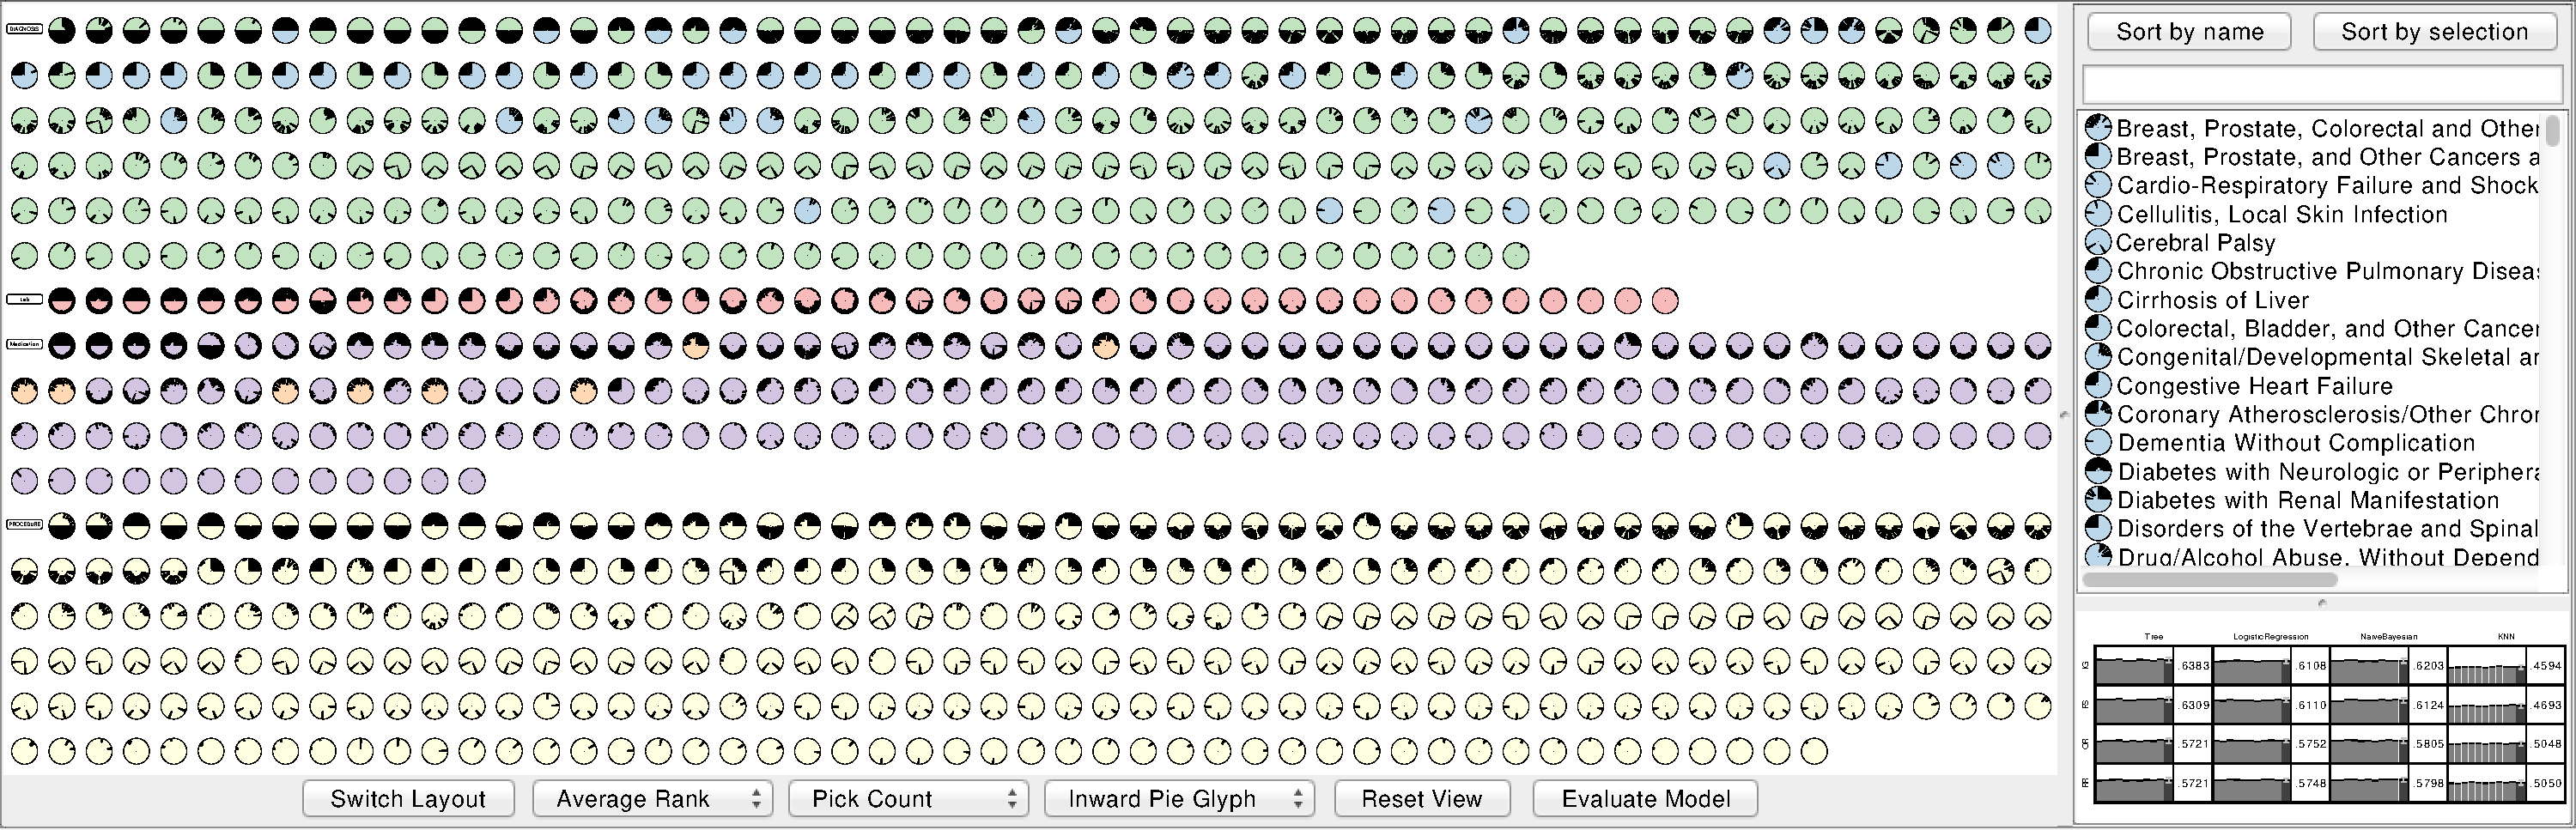
\includegraphics[width=\textwidth]{infuse/teaser}
\caption{
An overview of \infuse, a visual analytics tool that supports users to understand the predictive power of features in their models.  Each feature is ranked by various feature selection algorithms, and the ranking information is visualized in each of the three views within the system.  On the left, the Feature View provides a way to visualize an overview of all features according to their rank using a variety of layouts.  On the top-right, the List View provides a sorted list of all features, useful for selections.  On the bottom-right, the Classifier View provides access to the quality scores of each model.  Each of the views are coordinated, and users can brush between all three views.
}
\label{fig:teaser}
\end{figure*}

%% Uncomment below to disable the manuscript note
%\renewcommand{\manuscriptnotetxt}{}

%% Copyright space is enabled by default as required by guidelines.
%% It is disabled by the 'review' option or via the following command:
% \nocopyrightspace

% \begin{document}
% \section{Introduction}

% \maketitle

% !TEX root = ../featureselection.tex
\begin{figure*}[ht]
\centering
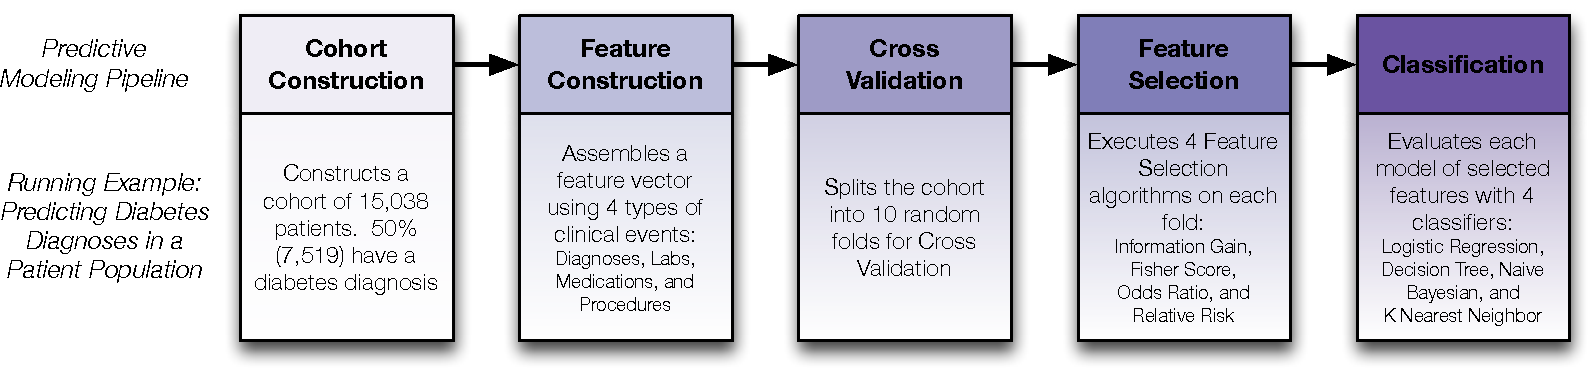
\includegraphics[width=\linewidth]{infuse/pipeline}
\caption{Steps of a typical predictive modeling pipeline.  For each step, we provide the details of the running example we use throughout the paper.
}
\label{fig:pipeline}
\end{figure*}

The visualization research community has usually focused on developing techniques and systems to support the analysis of datasets, with limited analysis of the relationship between datasets and the construction of models on top of them. However, there are a growing number of data scientists interested in more than just interpreting their data: they want to understand their data and predictive probabilities associated with them. Providing visual support for this kind of task has become important as many existing applications on the market and in scientific settings need to solve problems that are predictive in nature, e.g. prediction of customer behavior, diseases, drug effectiveness.

Predictive modeling is defined as the process of developing a mathematical tool or model that generates an accurate prediction \cite{kuhn2013applied}. However, building an accurate predictive model is far from trivial. First, modelers must construct cohorts, or distinct groups, to divide their datasets into cases and controls. Then, they must use a feature construction technique to define the feature vector. Next, they must define the parameters for cross-validation to ensure the results are statistically valid and robust. Then, they need to choose a feature selection algorithm to extract the informative features and include them in a model. And finally, they need to choose a classifier to evaluate the predictiveness of the model. For each of these decisions, there are a variety of techniques for cohort construction, feature construction, cross-validation, features selection, and classification to choose from, and there are currently no systematic guidelines to decide which algorithms are most appropriate for which types of datasets. Making the wrong choices can cause predictive models to fail. Kuhn and John argue that many predictive models fail because, ``predictive modelers often only explore relatively few models when searching for predictive relationships [...] due to either modeler's preference for, or knowledge of, or expertise in, only a few models or the lack of available software that would enable them to explore a wide range of techniques" \cite{kuhn2013applied}. We use these current limitations as motivation to research how visual analytics may improve the process of predictive modeling.

Our proposed research focuses on an important step in the predictive modeling pipeline: feature selection. When data is high-dimensional, feature selection algorithms are often used to remove non-informative features from models. Again, the analyst is confronted with the decision of which feature selection algorithm to utilize, and even if the analyst decides to try out multiple types, the algorithmic output is often not amenable to user interpretation. This limits the ability for users to utilize their domain expertise during the modeling process. To improve on this limitation, we developed \infuse (INteractive FeatUre SElection), a novel visual analytics system designed to help analysts understand how predictive features are being ranked across feature selection algorithms, cross-validation folds, and classifiers. We describe the tasks associated to the feature selection and understanding process and provide a design rationale for our solution. We also demonstrate, through case studies, how the system can lead to important insights for clinical researchers predicting patient outcomes from electronic medical records.

Concretely, our contributions include:

\begin{itemize}
\item A design and implementation of a predictive modeling exploration system,
\infuse, for understanding how predictive features are being ranked
across feature selection algorithms, cross-validation folds, and classifiers.
\item An Interactive Model Builder, where users can create customized models based on insights reached with \infuse, and then have their results evaluated in comparison to automated methods.
\item A case study of domain experts using
\infuse  to explore predictive models in electronic health records.
\end{itemize}

% The following text is taken from the PARAMO paper:
% "To develop an accurate and useful predictive model, a research- er generally needs to build and compare many different models as part of the discovery workflow. Each model can be viewed as an instance of the modeling pipeline and consists of a unique combination of the data, algorithms, and/or certain parameter configurations in the task components.
% A number of factors combine to increase the number of models that need to be explored, resulting in a large set of pipelines that have to be processed. First, the volume, variability, and heteroge- neity of EHR data require significant processing in building predic- tive models [10]. Second, there is uncertainty in knowing a priori which feature construction, feature selection, and classification algorithms are most appropriate for the specific target application [27]. As such, composition of an appropriate predictive model re- quires exploring a potentially large space of possible algorithms and parameters and their combinations. Third, for some biomedi- cal applications, the ability to interpret how the model works is just as, if not more, important than the accuracy of the model. Here, it is important to explore a variety of classification algo- rithms (e.g. decision trees, Bayesian networks, and generalized regression models) that produce trained models which can be interpreted by domain experts to verify and validate that the mod- el is clinically meaningful [28]. It is likely that multiple models can have similar performance in terms of prediction accuracy, but may differ significantly in their internal model parameters. By building multiple models, it becomes possible to select ones that have more clinically meaningful interpretations. Fourth, it is critical to statis- tically validate the models to ensure generalizability and accuracy. Cross-validation techniques can help with this endeavor, but can dramatically increase the number of models that need to be built and evaluated.""

\begin{figure*}[ht]
\centering
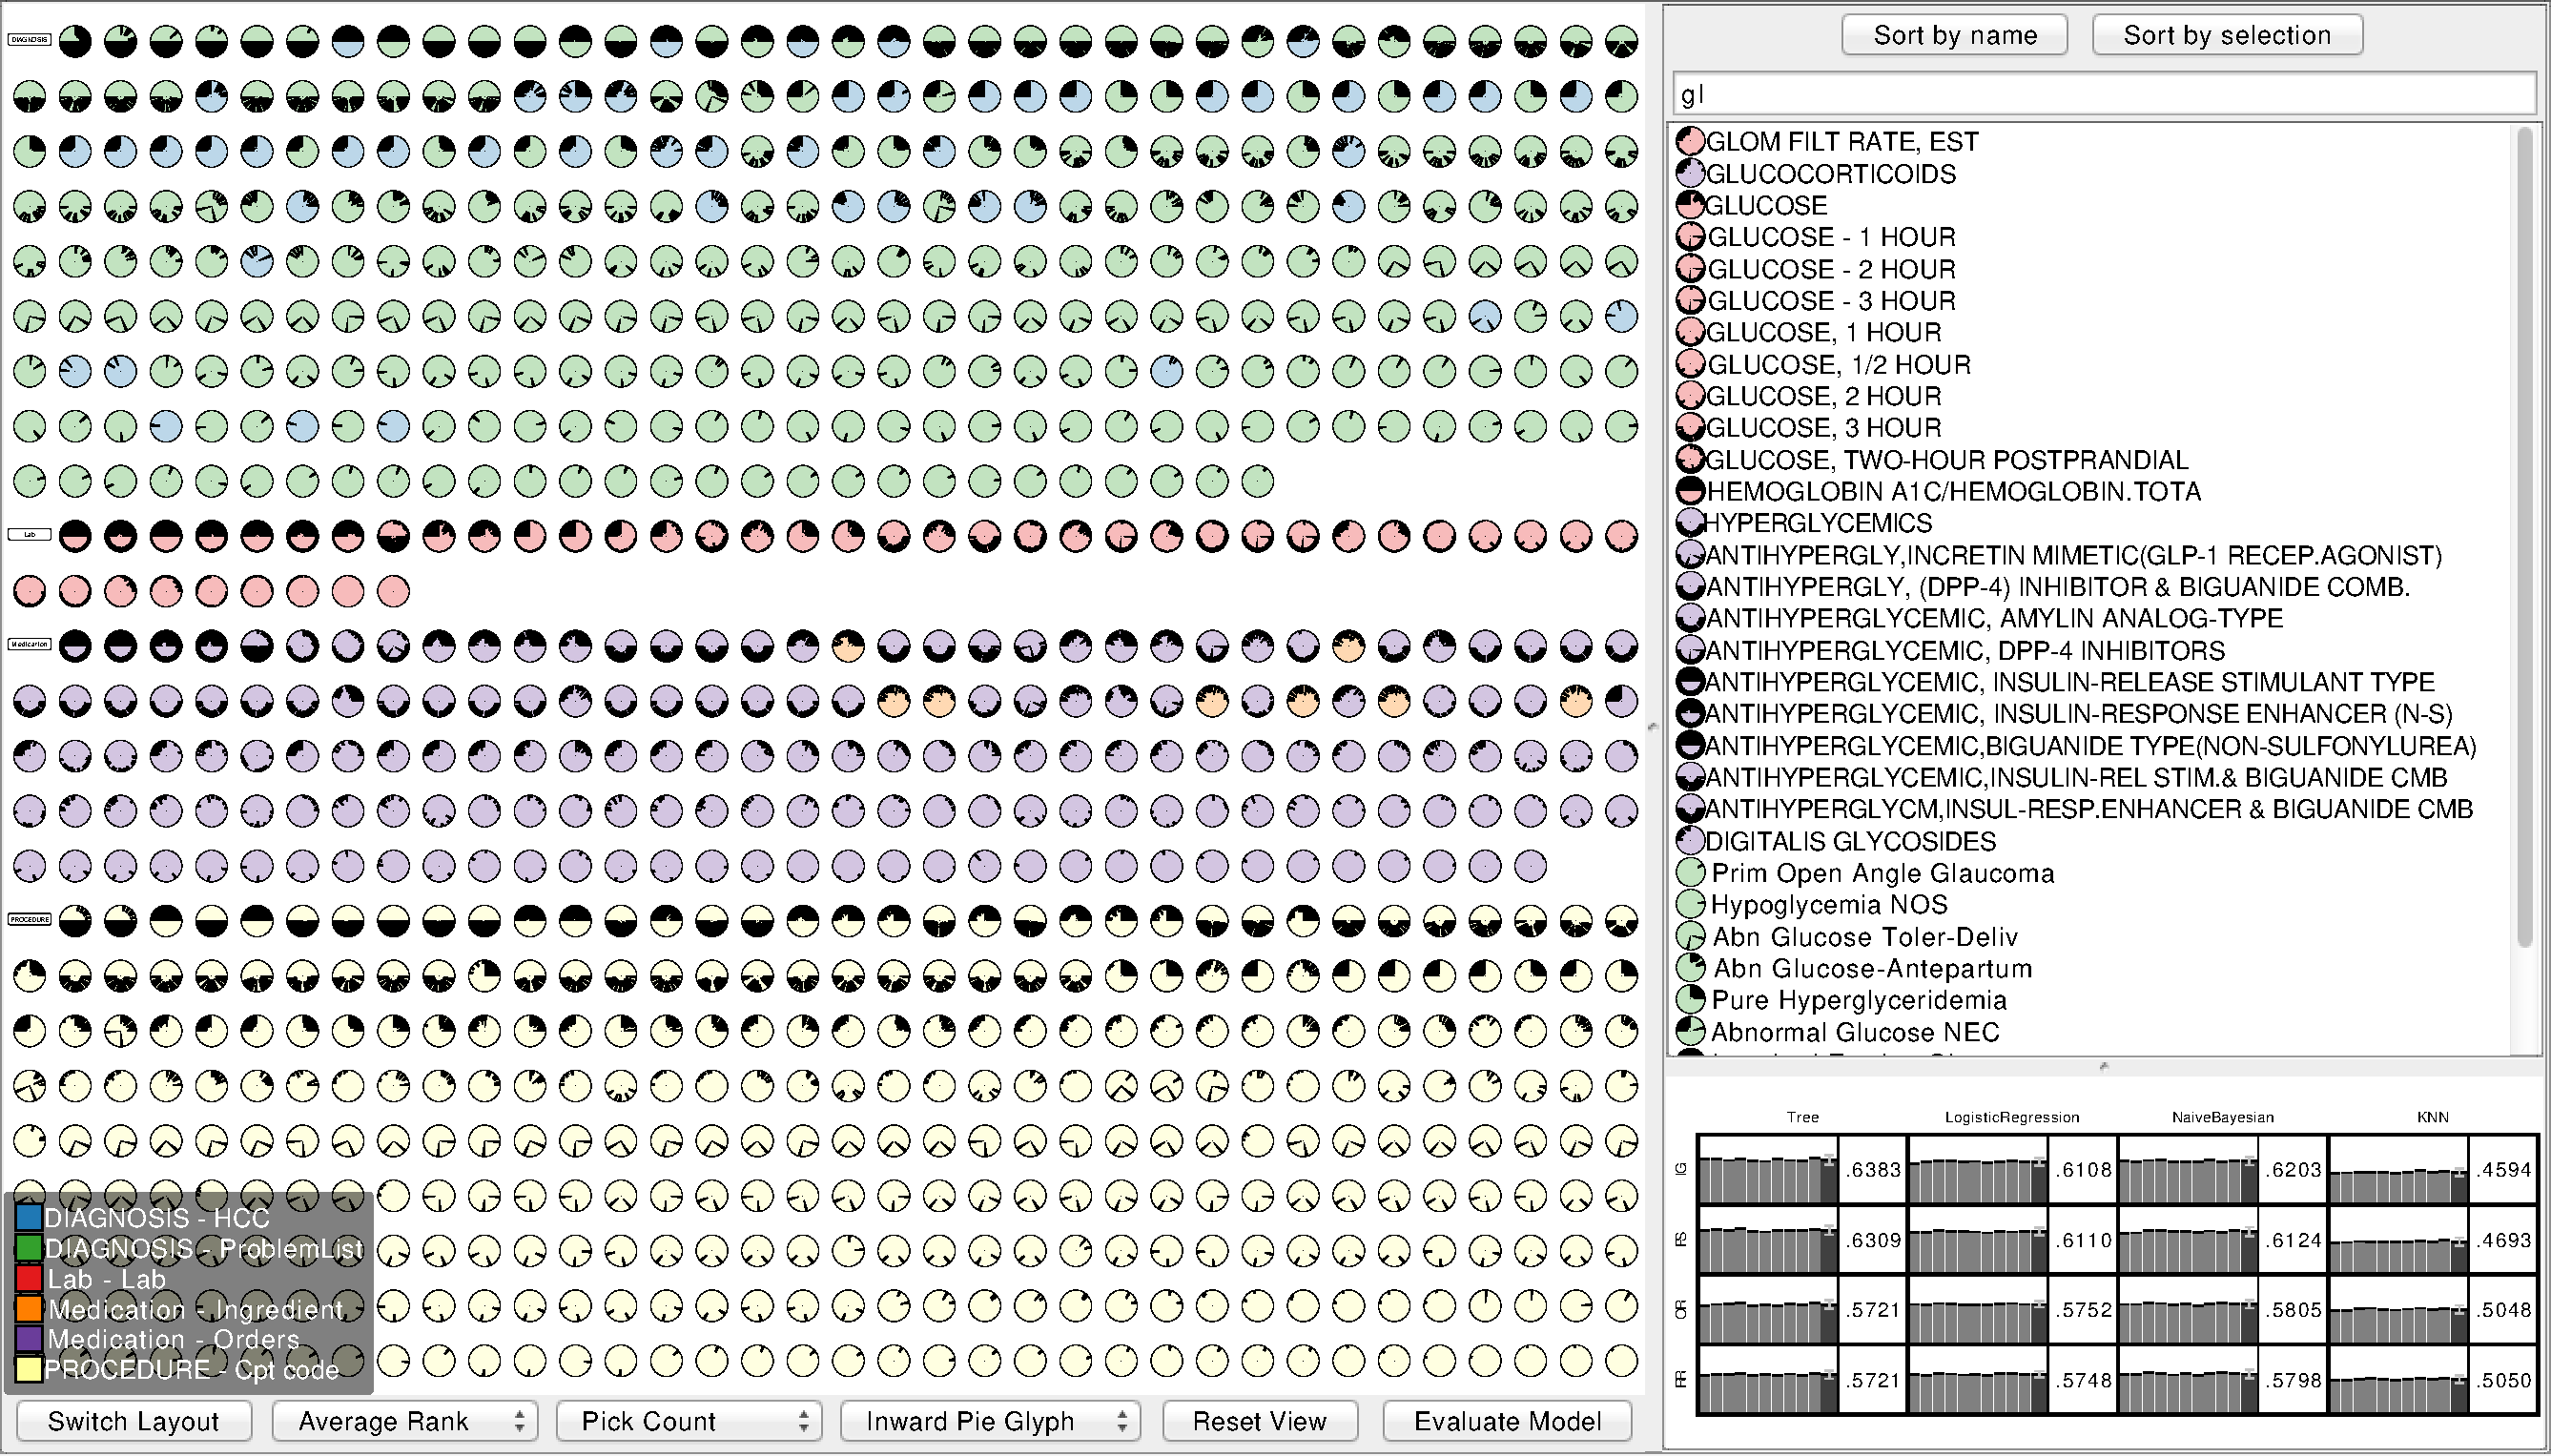
\includegraphics[width=\linewidth]{infuse/system}
\caption{
An overview of \infuse, a system for interactive feature selection.  On the left, the Feature View provides a way to visualize an overview of all features grouped by type and then sorted by importance.  The color key for the feature types and subtypes are shown at the bottom.  The buttons and combo boxes at the bottom can be used to switch layouts and define the axes of the scatterplot view shown in
Figure~\ref{fig:scatter}.  On the top-right, the List View provides a sorted list of all features, useful for selections.
This list can be filtered using the search box above. Currently only features containing the term ``gl" are shown.
The remaining features are sorted by the number and position
of the search term occurrences.
On the bottom-right, the Classifier View (Figure~\ref{fig:classifier}) provides access to the quality scores of each model.  Users can also select features and build custom models with the Interactive Model Builder.
}
\label{fig:system}
\end{figure*}

% !TEX root = ../featureselection.tex

\section{Motivation}

\subsection{Predictive Modeling in Health Care}
\label{sec:motivation_healthcare}
Predictive modeling is a common and important methodology used
in medical informatics and health care research.
For instance, it can be used to detect diseases in patients early
before they progress \cite{bellazzi2008predictive} and to
personalize treatment guidelines to understand which populations
will benefit from an intervention \cite{jensen2012mining}.
In order to derive such insights and build successful predictive models,
it is common for health care researchers to implement, evaluate,
and compare many models with different parameters and algorithms.
A common workflow for predictive models is a 5-step process,
illustrated in Figure~\ref{fig:pipeline}:
(1) cohort construction, (2) feature construction, (3) cross-validation,
(4) feature selection, and (5) classification.
There are currently few tools that support this complex
workflow for predictive modelers.

A recent platform, PARAllel predictive MOdeling (\textit{PARAMO}) \cite{paramo},
enables users to specify a small number of high-level parameters
to support this 5-step workflow.
\textit{PARAMO} then uses Map-Reduce to execute these many tasks in parallel.
After the models have been constructed and evaluated by classifiers,
users can compare area under curve (AUC) scores of different models and select the
ones with the highest predictive power.
While this ability to construct and evaluate models at scale is
an important breakthrough for clinical researchers, the clinical
experts are still left out of the loop at each of these 5 stages,
as each of the algorithms act as a black box.

This type of workflow limits the ability of clinical researchers to use
their domain knowledge to assist in the model building phase.
While multiple models may have similar performance in terms of
prediction accuracy, there is a desire to ensure that models
with more clinically meaningful features are selected
\cite{chen2006medical}.

\subsection{Running Example: Diabetes Prediction}
\label{sec:running_example}
In order to make our contributions concrete, we
utilize a running example from our case study.
Our case study involves a team of four clinical researchers interested
in using predictive modeling on a longitudinal database of
electronic medical records. The research team consisted of one MD researcher with a background in emergency medicine, and three PhD researchers with backgrounds in health care analytics.
Their database features over 300,000 patients from a major
health care provider in the United States.
The team is interested in building a predictive model to predict if a patient
is at risk of developing diabetes, a chronic disease of high blood sugar levels
that causes serious health complications.

From this database, the team constructs
a cohort (Step~1) of 15,038 patients.
50\% of these patients (7,519) are considered
incident cases with a diagnosis of diabetes.
Each case was paired with a control patient based on
age, gender, and primary care physician resulting
in 7,519 control patients without diabetes.
From the medical records of these patients,
they extract four meaningful types of features (Step~2): diagnoses,
lab tests, medications, and procedures.
In total, there were 1,627,736 diagnosis events (6,709 unique types), 361,026 lab events (193 types), 818,802 medication events (344 types), and 853,539 procedures (4,403 types).
For our visualization, we only consider types of features that were picked
by feature selection algorithms which results in 859 features to display.

Next, in order to reduce the bias of the predictive models,
the team uses 10 cross-validation folds (i.e. random samples) (Step~3) to divide the
population randomly into 10 groups.
After cohorts, features, and folds are defined, the
clinical researchers are ready to use feature selection.
The team has four feature selection algorithms implemented
and available to them (Step~4): these include \textit{Information Gain}
and \textit{Fisher Score}, which have been used extensively by the researchers,
as well as two new ones which were recently implemented by
their technologists: \textit{Odds Ratio} and \textit{Relative Risk}.
Finally, the team evaluates each selected feature set as a model using
four classifiers (Step~5): \textit{Logistic Regression}, \textit{Decision Trees},
\textit{Naive Bayes}, and \textit{K-Nearest Neighbors}.

Typically, this team executes a pipeline of multiple feature selection
algorithms, and chooses the model that ends up
with the best scores from the classifier.
Although this team has an interest in embedding domain knowledge
into their models, their current platform for running predictive models
does not have a user interface where users can view or edit the
specific features that make up each model.
Therefore, resulting models are typically not interpretable
by domain experts,
and do not support bringing in their medical expertise by prioritizing or removing features that may not be relevant to the disease they are modeling.

\subsection{Task Analysis}
\label{sec:task-analysis}

The data analysis team initially expressed an interest of having a visual analytics system to aid them in making sense of the complex information generated by the modeling pipeline. During our interviews we agreed to focus on the feature selection and classification steps, as they needed visualizations to reason about the effects of choosing different combinations of the available algorithms. Without such visualizations, the researchers ability to choose among different algorithms is ineffective.

Through our interactions with the analysts we derived three main tasks that guided the design of \infuse:


\begin{description}
\item[Task1 - Comparison of feature selection algorithms.] In data sets with thousands of features, it is important to have a quick way to understand how feature selection algorithms rank different features differently. Some of the typical questions the researchers ask are: ``\textit{Which features are consistently ranked highly by all the algorithms?}"; ``\textit{How much do the algorithms differ in their ranking?}"; ``\textit{Are there features that have a high rank with some algorithms and a low rank with some others?}"; ``\textit{How robust are the rankings with respect to different data samples?}"

\item[Task 2 - Comparison of classification algorithms.] The output of each feature selection algorithm is used to feed a series of classification algorithms. At the end of this process, the user is left with a $F \times C$ number of performance comparisons, where $F$ is the number of feature selection algorithms and $C$ the number of classification algorithms. Typical questions our researchers ask are: ``\textit{Which combinations of feature selection and classification algorithms give the best scores?}"; ``\textit{Are there feature selection algorithms that score consistently better across the set of classification algorithms?}"; ``\textit{Are there classification algorithms that score consistently better across the set of feature selection algorithms?}"; ``\textit{Which sets of features are selected in the model(s) that give the highest performance?}"

\item[Task 3 - Manual selection and testing of new feature sets.] Related to the last question of Task 2, the researchers see value in being able to add or remove features of interest from models. This is desired because there can be additional domain-relevant knowledge, beyond model performance, to introduce a desired feature or remove an undesired one.  Typical questions our researchers ask are: ``\textit{How does the performance of the model increase or decrease if I remove or add these features?}"; ``\textit{How does a new model compare to the models automatically built by the system?}"
%;``\textit{How predictive is a single feature?}"
%;``\textit{Could switching to a different lab-test yield similar performance while being less expensive?}".
\end{description}


\infuse was designed to support these three tasks by providing a visualization of large sets of features and how these features are used by the modeling algorithms. After several design iterations, we converged on a visual design where features are first-class citizens of the visual representation: that is, each visual object in the main view represents a feature and its design and layout reflects information obtained from the algorithms.  A representation centered on features aligns well with the analysts' mental model and makes features easily identifiable through their names. Each feature, in fact, represents real-world entities like medications, lab tests and diagnoses, that have rich semantics and can be easily identified and understood by domain experts.

% !TEX root = ../featureselection.tex

\section{Related Work}
While visualization of multidimensional data has traditionally focused
more on the visualization of the data space, visualizing data features
has important applications in real-world scenarios;
especially when confronted with hundreds or even thousands of dimensions.
In this context, visualization helps data analyst making sense of the
feature space while including their background knowledge in the process.
Visual feature selection can, for instance, help rank features according
to predefined scores, detect similarities among dimensions
(thus gauging intrinsic dimensionality of feature spaces),
merge or combine features into composite features.
In the following we review visualization literature that consider
the specific problem of visualizing large sets of features.

\subsection{Visual Feature Selection}
%\enrico{I am wondering if there is a way to structure these techniques into some classes. For instance some are more into finding similarities and groups of dimensions others are more into ranking.}

Several approaches to feature selection and dimensionality reduction, in general, exist in visualization.
The early work of Guo~\cite{Guo2003} introduced the idea of
visualizing relationships between features sets.
His system is based on an interactive matrix view where rows and
columns represent features and the cells are colored according to
feature similarity (calculated as entropy and ${\chi}^2$).
The matrix is automatically sorted to allow selection of subspaces
(feature subsets) where data shows interesting clusters.
Visual hierarchical dimension reduction \cite{wang2003interactive}
allows detection and grouping of similar features as well.
The technique is based on a hierarchical clustering algorithm
which clusters dimensions in terms of their similarity and present
them in a \textit{sunburst} visualization \cite{yang2003interactive}.
Users can interactively choose an aggregation level and use the aggregated
dimensions to display data with the reduced set of dimensions.
Johansson and Johansson \cite{Johansson2009} present an integrated environment based on
\textit{parallel coordinates} visualization where the number and order of
dimensions (axes) presented at any time is guided by a ranking algorithm
that takes into account associations as well as intrinsic interestingness of
each feature to interactively choose how many features to visualize.
Similar in spirit is the \textit{rank-by-feature} framework \cite{seo2005rank} in which
the data features are organized, ranked and visualized in
1D and 2D visual representations
(e.g. histograms, bar charts and scatterplots).
The user can for instance inspect a matrix of feature pairs,
ranked by one of the available ranking functions, and single
out those that show interesting associations.
A similar mechanism is also used in \textit{scagnostics} \cite{wilkinson2005graph} a
quality metric approach \cite{bertini2011quality} that ranks axis pairs according to the pattern/shape they create in a scatterplot visualization.

More similar to the solution presented in this paper are visualizations that
focus on plotting dimensions as data points in the visual representation
(rather than, for example, as axes of a visualization where the data
items represent records of a data table).
\textit{Value and Relation Display} visualizes data features as icons
in a scatter plot visualization \cite{YangPHMWR04}.
The icons are positioned using a \textit{multidimensional scaling}
algorithm which positions dimensions with
similar distributions close together.
The icons are designed to represent the distribution of the
data values within the feature.
Such a display allows to detect groups of similar dimensions
and to construct multidimensional visualizations by subsetting
the original feature space.
\textit{Brushing Dimensions} \cite{Turkay2011} is a similar approach
where data features are plotted as dots in a scatter plot using
descriptive statistics as axes (e.g. variance, median, kurtosis).
The plot is paired with a data item scatter plot which allows for data
and feature linking and exploration.

All of the methods described above are based on the calculation
of statistical parameters from the data as a way to characterize
and expose relationships between the features.
Our approach differs in that \infuse interacts directly
with feature selection and classification algorithms to help in
the discovery of predictive feature sets.
A similar approach is found in \textit{SmartStripes} \cite{May2011},
a visual analytics system that allows tight interaction between feature selection algorithms and visualization. Our system differs in that our focus is on the comparison of the output of multiple feature selection algorithms rather than a single one.



%\joschi{\cite{Guo2003} interactive feature selection -- entropy matrix etc}
%\joschi{\cite{Ingram2010} creating workflow for feature reduction}
%\joschi{\cite{Johansson2009} interactive dim reduction via user defined weighting}
%\joschi{\cite{Kidwell2008} visualizing partially ranked data}
%\joschi{\cite{May2011} guiding fs with interactive system}
%\joschi{\cite{YangPHMWR04} features as points in scatterplot -- high dimension exploration -- MDS of correlation as layout}
%\joschi{\cite{Seo2005} rank by feature -- dendogram, scatterplot, matrix, list view}
%\joschi{\cite{Turkay2011} brushing dimensions}

%\enrico{Other things we might want to include is subspace visualization as in a way it deal with the problem of finding feature subsets. E.g., Work from myself and from Wilkinson at VAST.}
%\joschi{PARAMO \cite{paramo}}
%\enrico{Should we briefly review feature selection strategies and algorithms as well?}

\subsection{Visualization in Predictive Modeling}
%\cite{kuhn2013applied} for examples of other predictive modeling systems.}

%\adam{should we put general interactive machine learning techniques, e.g. Amershi, S., Fogarty, J., Kapoor, A., and Tan, D.(2011) Effective End-User Interaction with Machine Learning. In Proceedings of the AAAI Conference on Artificial Intelligence (AAAI 2011), Nectar Track, pp. 1529-1532.}
%\enrico{Yes, now I realized there is quite some stuff to cite here. Some work on interactive visual classification from Ankerst and Kwan Lu Ma. SOme recent work at VAST. Some stuff from the MSR folks.}

Visualization has also been used to aid in the creation of predictive models, not only in the selection of features that might be helpful in constructing such models. Visual construction and assessment of decision tree models have been the subject of a good number of works in the field. Ankerst \emph{et al.}, introduced the idea of using pixel-based visualization as a way to manually construct decision trees by giving the user the ability to observe class distributions within each node and to interactively select splitting points \cite{ankerst1999visual, ankerst2000towards}. A similar idea is proposed in \textit{PaintingClass} a visualization technique to manually build a decision tree through interaction of parallel coordinates and multidimensional scaling techniques to identify coherent groups of multidimensional data \cite{Teoh:2003:PIC:956750.956837}. More recently, \textit{BaobabView} has been presented as a system to inspect and validate a classification model through a tree representation. The paper presents a thorough analysis of the number of tasks that visualization can support in this area and how they are covered by the proposed system \cite{van2011baobabview}.

While all the aforementioned systems focus largely on decision trees, visualization has been used in other classification and regression systems that leverage other prediction models. The \textit{iVisClassifier} \cite{choo2010ivisclassifier} for instance uses \textit{linear discriminant analysis (LDA)}, a supervised dimensionality reduction method, to project multidimensional data in a scatterplot visualization taking into account information provided by the data labels. The technique allows to visually link the high-dimensional structure to the low-dimensional representation and build clusters. The clusters are then used to classify new data that is progressively introduced into the system to refine the model. Steed \emph{et al.}, in their \textit{cyclone trend analysis} provide a parallel coordinates visualization that leverage computational analysis to identify features with high predictive power in stepwise regression tasks and allows to build predictive models for multidimensional climate data \cite{steed2009guided, steed2009tropical}. Recently, a visual analytics system for regression analysis has been proposed by M\"uhlbacher and Piringer \cite{muhlbacher2013partition}. The system is more similar to our work in nature as it also focuses on the predictive power of feature sets and guides the user in the predictive modeling process. The main difference between this work and ours is our focus on classification rather than regression models and the use of multiple feature selection and classification models to better understand how features score across multiple models.


% !TEX root = ../featureselection.tex

\vspace*{1em}

\section{INFUSE}
\label{sec:infuse}

In this section, we describe the design of \infuse, which aims to assist predictive modelers with the tasks introduced in Section~\ref{sec:task-analysis}. By providing visualizations for users to interpret the results of feature selection algorithms, as well as the ability to customize the models with domain knowledge that may have been missed by the automated algorithms, \infuse provides a user-centric way of manipulating predictive models.

\begin{figure}[ht]
\centering
\hspace*{0.02\linewidth}%
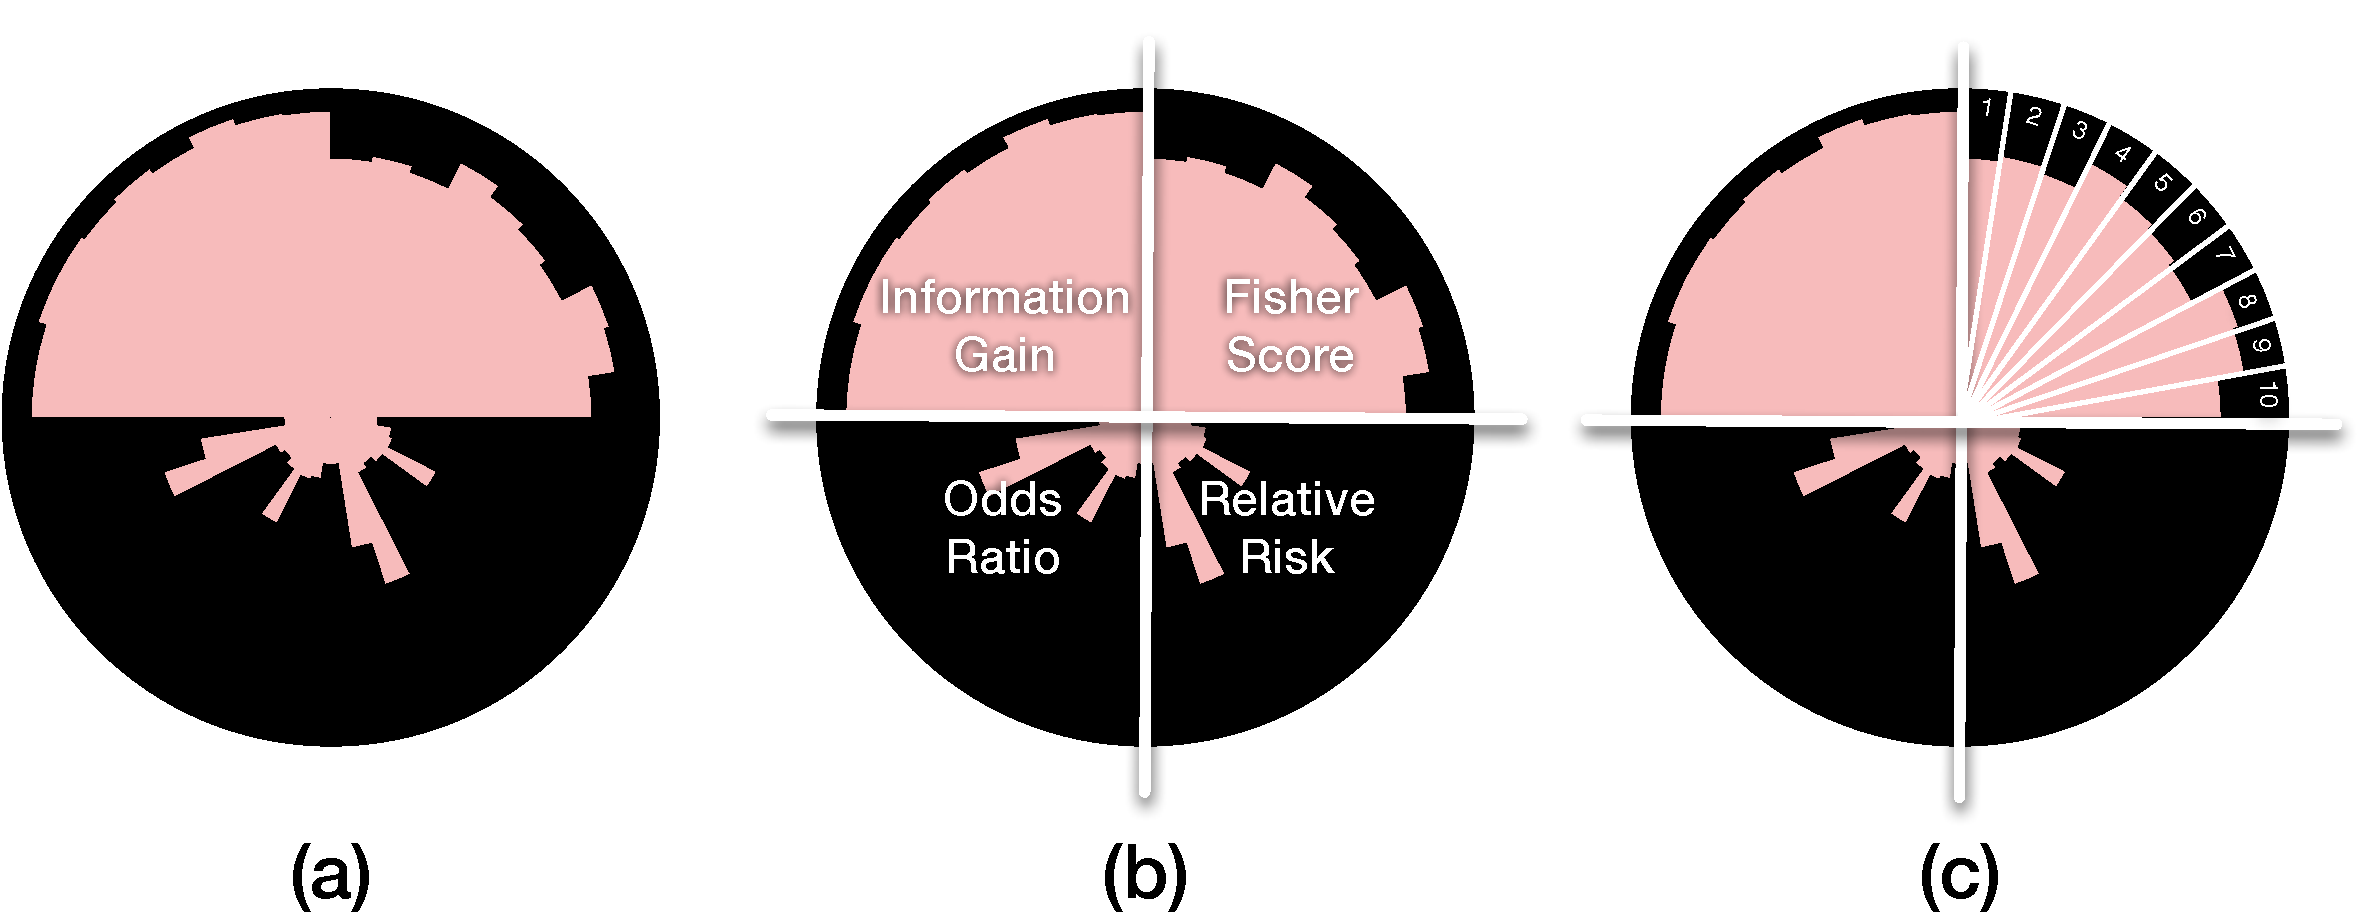
\includegraphics[width=0.95\linewidth]{infuse/glyph-key}
\caption[How to read the glyph representation of \infuse.]{
(a) The glyph representation of a feature in the \infuse system.
(b) Multiple models for each feature are represented as \emph{model sections}.  In this example, the feature is divided into four sections, as it was ranked by four feature selection algorithms (Information Gain, Fisher-Score, Relative Risk, and Odds Ratio.).
(c) Each section is further divided into \emph{fold slices} representing each of the cross-validation folds. Each fold slices features a inward-filling bar that represents the rank of this feature in that fold.
A longer bar implies the feature has a better rank.  If no bar appears, the feature was unranked in the fold, and thus did not meet the importance threshold.
\vspace*{2em}
}
\label{fig:glyph-key}
\end{figure}

\begin{figure}[ht]
\begin{subfigure}{0.23\linewidth}
\centering
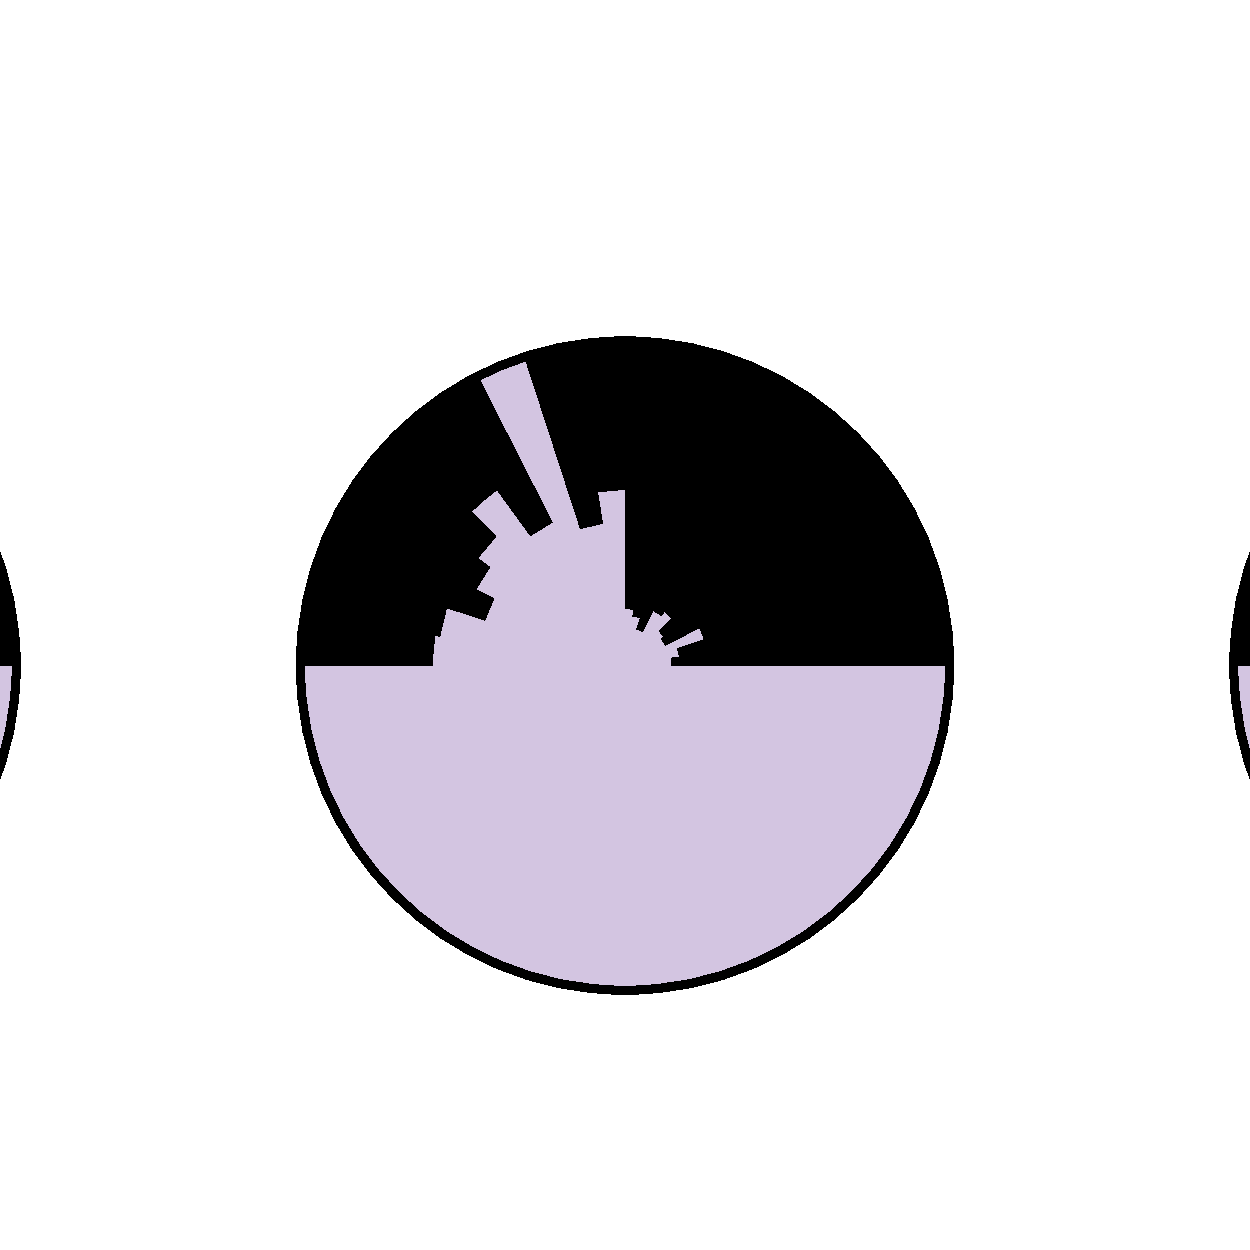
\includegraphics[width=\linewidth,clip,trim={2.4cm 4cm 1.7cm 4cm}]{infuse/g0}
\caption{}
\label{subfig:inward}
\end{subfigure}%
\hspace*{0.01\linewidth}%
\begin{subfigure}{0.23\linewidth}
\centering
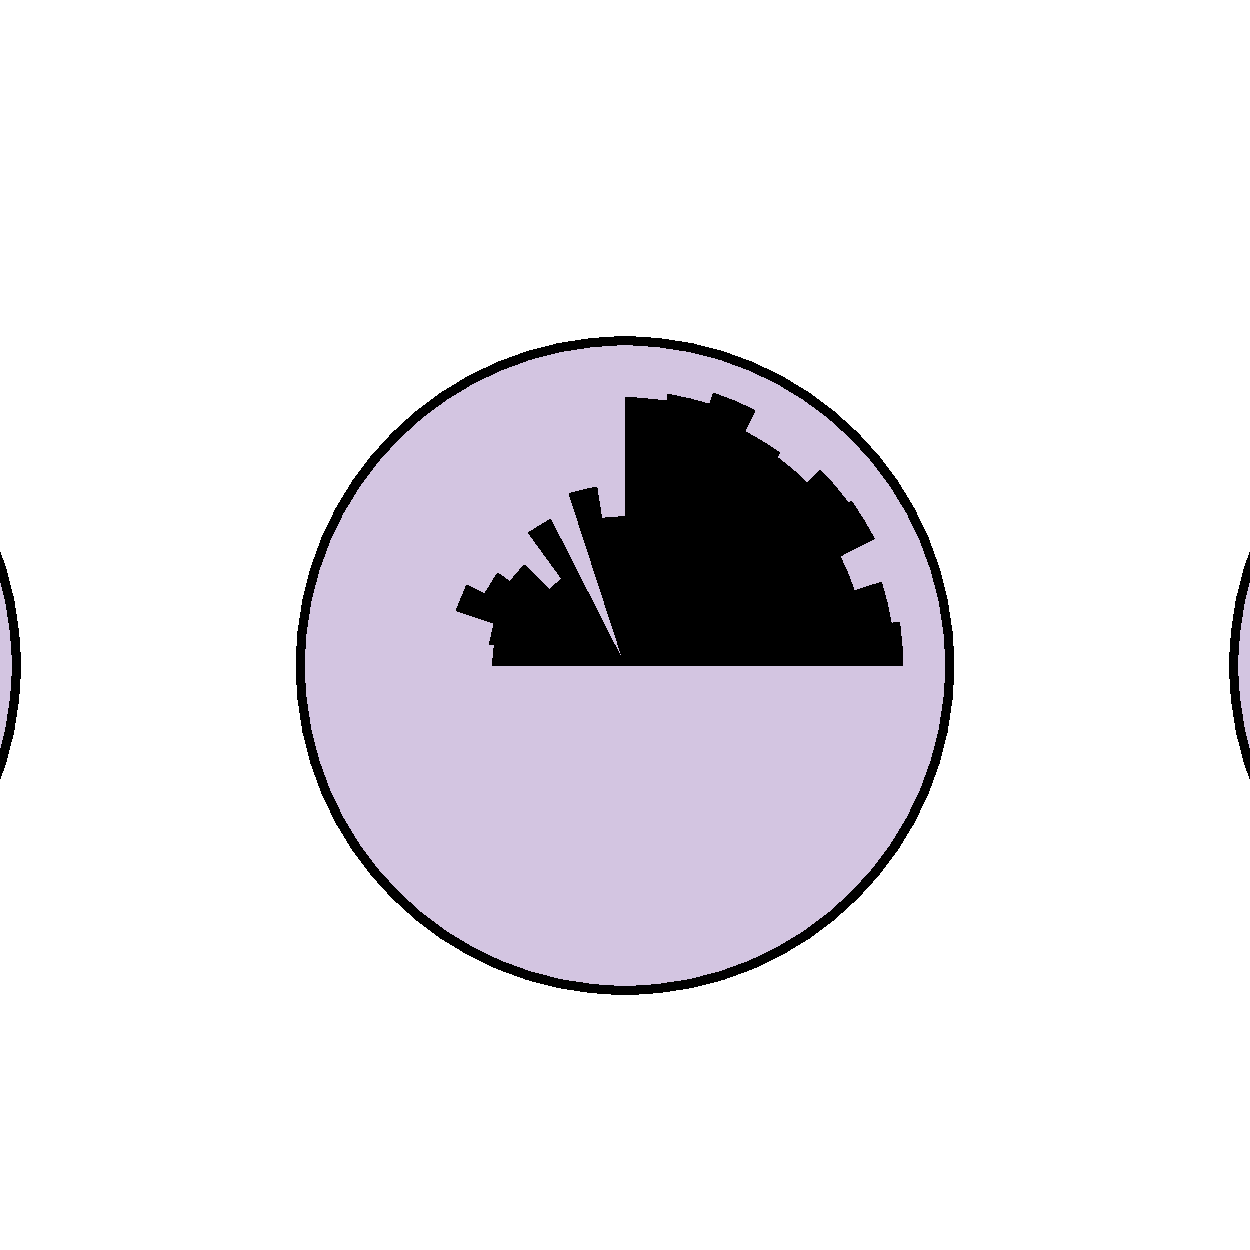
\includegraphics[width=\linewidth,clip,trim={2.4cm 4cm 1.7cm 4cm}]{infuse/g1}
\caption{}
\label{subfig:pie}
\end{subfigure}%
\hspace*{0.01\linewidth}%
\begin{subfigure}{0.23\linewidth}
\centering
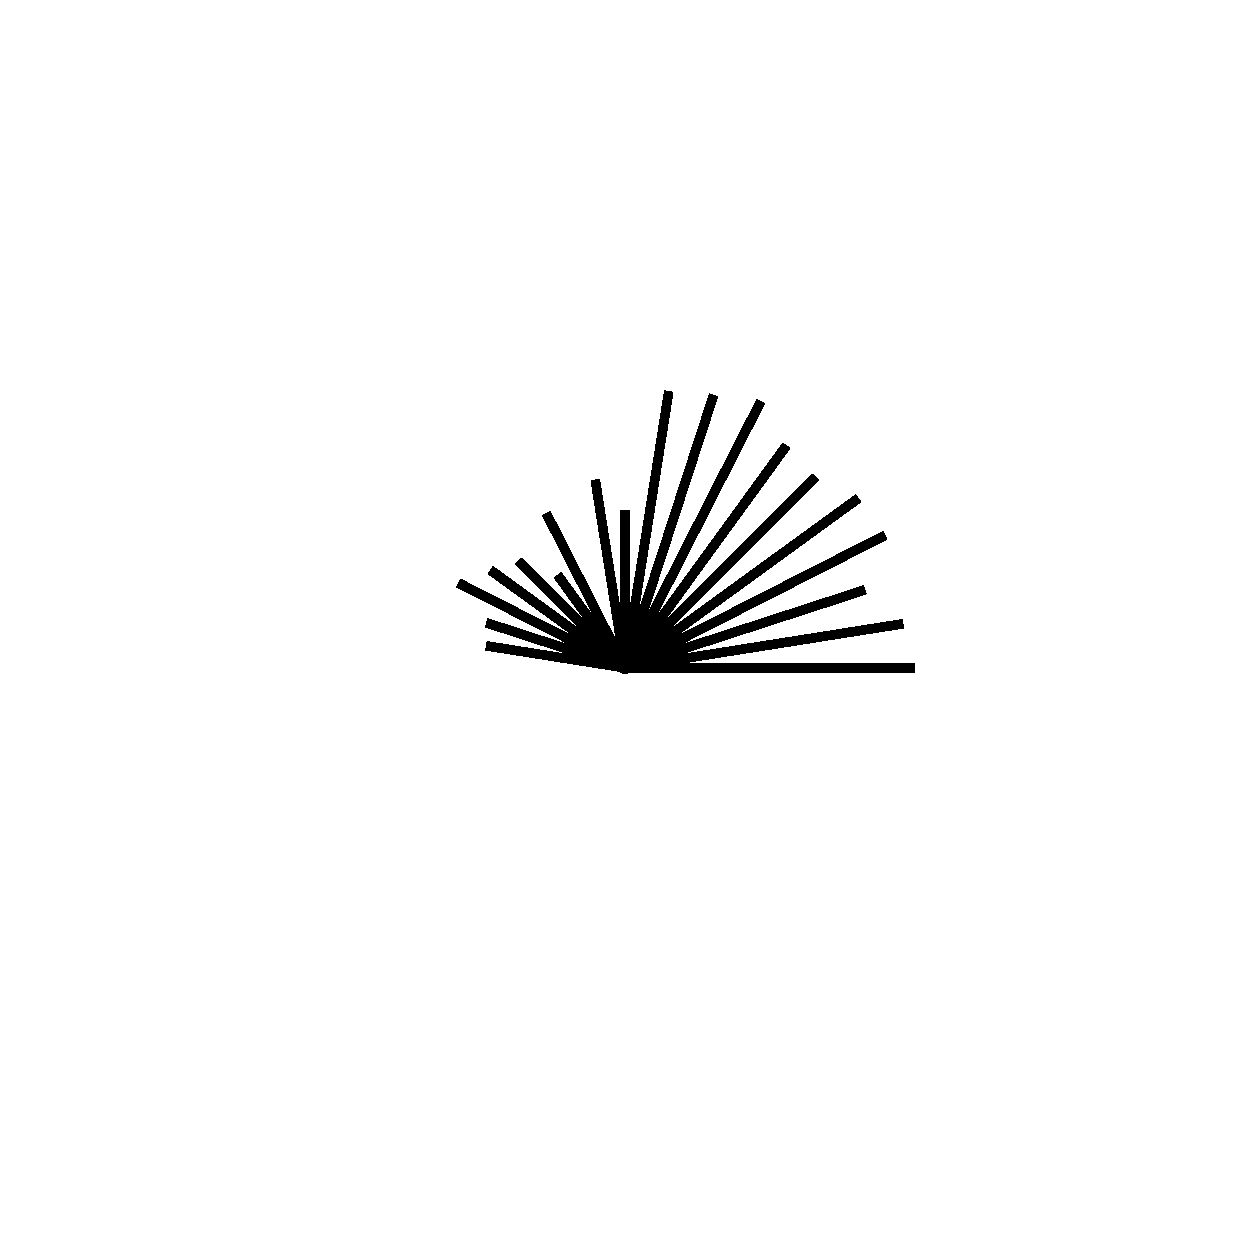
\includegraphics[width=\linewidth,clip,trim={2.4cm 4cm 1.7cm 4cm}]{infuse/g2}
\caption{}
\label{subfig:star}
\end{subfigure}%
\hspace*{0.01\linewidth}%
\begin{subfigure}{0.23\linewidth}
\centering
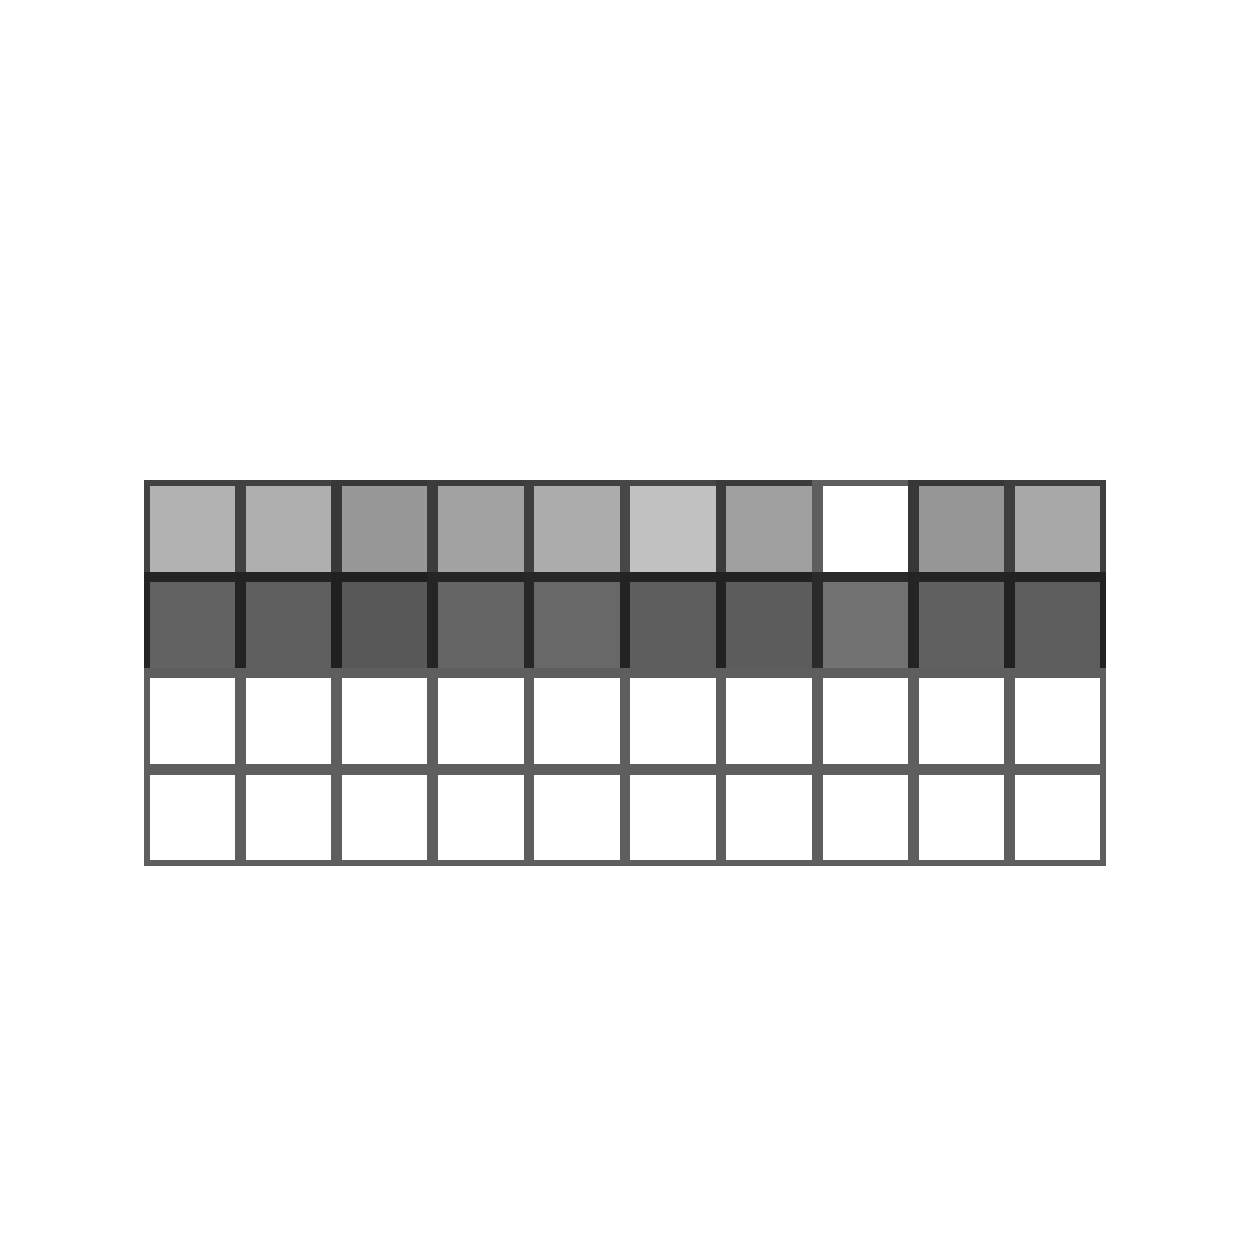
\includegraphics[width=\linewidth,clip,trim={2.4cm 4cm 1.7cm 4cm}]{infuse/g3}
\caption{}
\label{subfig:matrix}
\end{subfigure}%
\caption[Different glyph designs.]{
Different glyph designs.
\subref{subfig:inward} shows \emph{fold slices} with bars growing from perimeter to center
whereas \subref{subfig:pie} grows from center to perimeter.
\subref{subfig:star} shows a typical starburst glyph and
\subref{subfig:matrix} shows a matrix using luminance to show the ranks.
Note that in \subref{subfig:pie} and \subref{subfig:star} it is difficult
to see that this feature is unranked in the third fold from the right in
the top left quadrant.
The values in \subref{subfig:star} are difficult to read because
there is no reference to how big the values are.
Luminance, as used in \subref{subfig:matrix} is a harder perceptual attribute for users
to interpret and distinguish than length and area are, as used by the other glyphs.
}
\label{fig:glyph_design}
\end{figure}

\subsection{Data and Design}

We provide a brief overview of data types utilized by the system. A predictive model, in our setting, is a model trained and validated with machine learning using a high number of features as an input to train the model. These features are the primary data items of \infuse. Each feature has a label representing the feature name (e.g. Diabetes), a category to which the feature belongs to (e.g. Diagnosis), and a subtype (e.g. Problem List, the health problems that led to the diagnosis).

Feature selection algorithms receive as an input the whole set of existing features and return a subset of features selected and ranked according to their estimated predictive power. Since in our setting we use the output of multiple algorithms at once, each feature can further be described by the rankings they receive from all these algorithms (where features that are not selected are marked as unranked). Furthermore, since cross-validation is used, each feature actually gets ranked multiple times by each algorithm, leading to a total number of $\#\textit{feature selection algorithms} \times \#\textit{folds}$ ranks that quantitatively describe each feature.


%As described above in \ref{sec:motivation_healthcare}, feature selection works the features can be ranked by multiple feature selection algorithms, across multiple cross-validation folds. More precisely, for a pre-defined set of feature selection algorithms, each feature can further be described by the which results in number of ranks per feature. If a feature is not selected by a feature selection algorithm, it means it did not reach the threshold to be considered information and is unranked.

The predictive models built using the output generated by feature selection also provide useful information that we use in our system. Each feature set generated by the process described above is used as an input to a classification algorithm. The algorithm builds a model that corresponds to the specific pair of feature set and classification algorithm used for its training. The classifier, in turn, can be described in terms of its performance using the Area Under Curve (AUC), a measure that is commonly used by modelers to give numerical performance scores to models \cite{kuhn2013applied}.

%Each model within a cross-validation fold is then scored by multiple classification algorithms in the form of AUC (the Area Under Curve of the false positive rate in relation to the true positive rate) scores.  The overall quality of a feature set is the average area under curve for all used classification algorithms.

The primary goal of \infuse is to visualize this information so that users can understand the predictive power of features in their models. The user interfaces is organized around three main coordinated views as shown in Figure~\ref{fig:system}: the \textit{Feature View} provides a way to visualize an overview of all features providing information about their attributes and ranking received from feature selection; the \textit{List View} provides a sorted list of all features to get easy access to their labels and to assist the user in searching features according to some predefined criteria like their name or category; the \textit{Classifier View} provides access to the quality scores of each model built using the process described above. The views are coordinated so that selections in one view are propagated to all the other views. In the following we provide additional information about the design of each view.

% Seeing how features perform in various models
% is important for our system.
% Therefore, features showing their ranks in different models are
% first-class citizens of the visualization and for every feature
% the ranks can be seen at any time.
% Features can also be selected by the user to see or build feature sets.
% Selections are linked and visible throughout the tool.

% The system is split into three main components.
% The central part is the feature view that shows all features
% with their ranks as glyphs.
% The positions of the features can be sorted by type and
% overall importance to get an overview or they can
% be positioned on a scatterplot to show additional data about them.
% The type and subtype can be inferred from the glyph.
% Further information about a feature, like name,
% statistics about the rankings which are used as axes for the scatterplot,
% and exact rank numbers can be displayed as tooltip.

% Features are also shown in the list view on the right side.
% This view focuses more on the names of the features but
% shows also the glyph as orientation.
% The order of the elements in the list can be chosen to be by type,
% subtype, and then name, or by showing currently selected features on
% top, ranked by their importance.

% Seeing the area under curve for different
% feature sets is also an important task, since the quality
% of those sets is measured by it.
% In the bottom right corner the area under curve of all models
% is shown for every classification algorithm as matrix.
% Models can be picked to select the features of the corresponding set.

\begin{figure*}[ht]
\centering
\begin{subfigure}{0.24\linewidth}
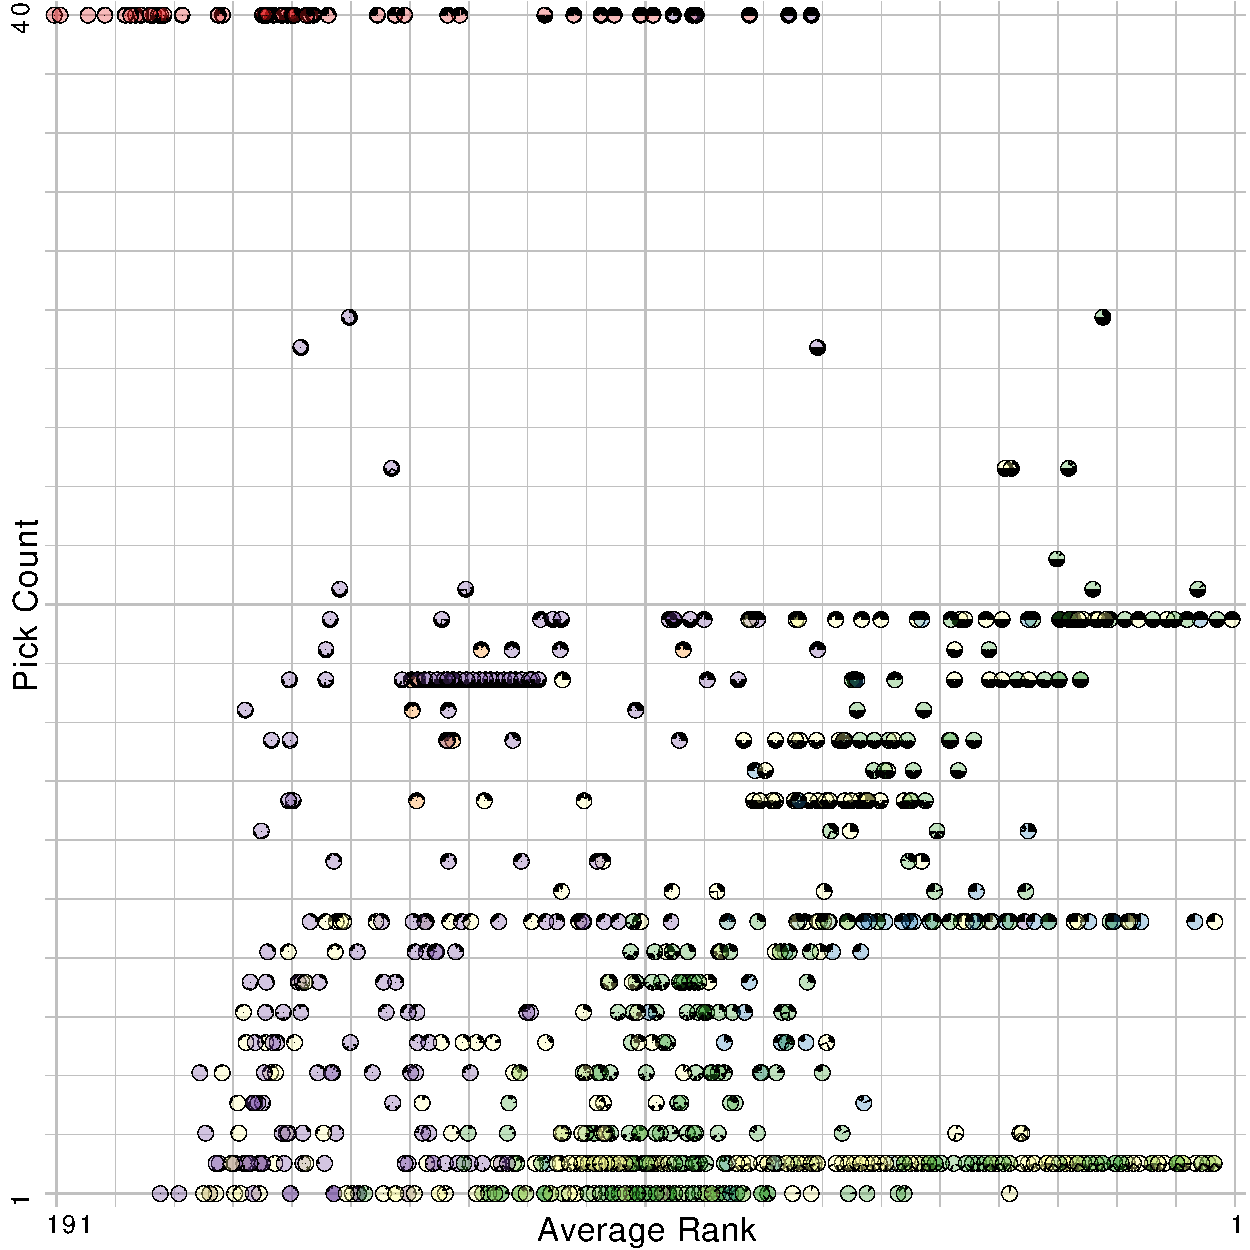
\includegraphics[width=\linewidth]{infuse/ap}
\label{subfig:ap}
\end{subfigure}%
~%
\begin{subfigure}{0.24\linewidth}
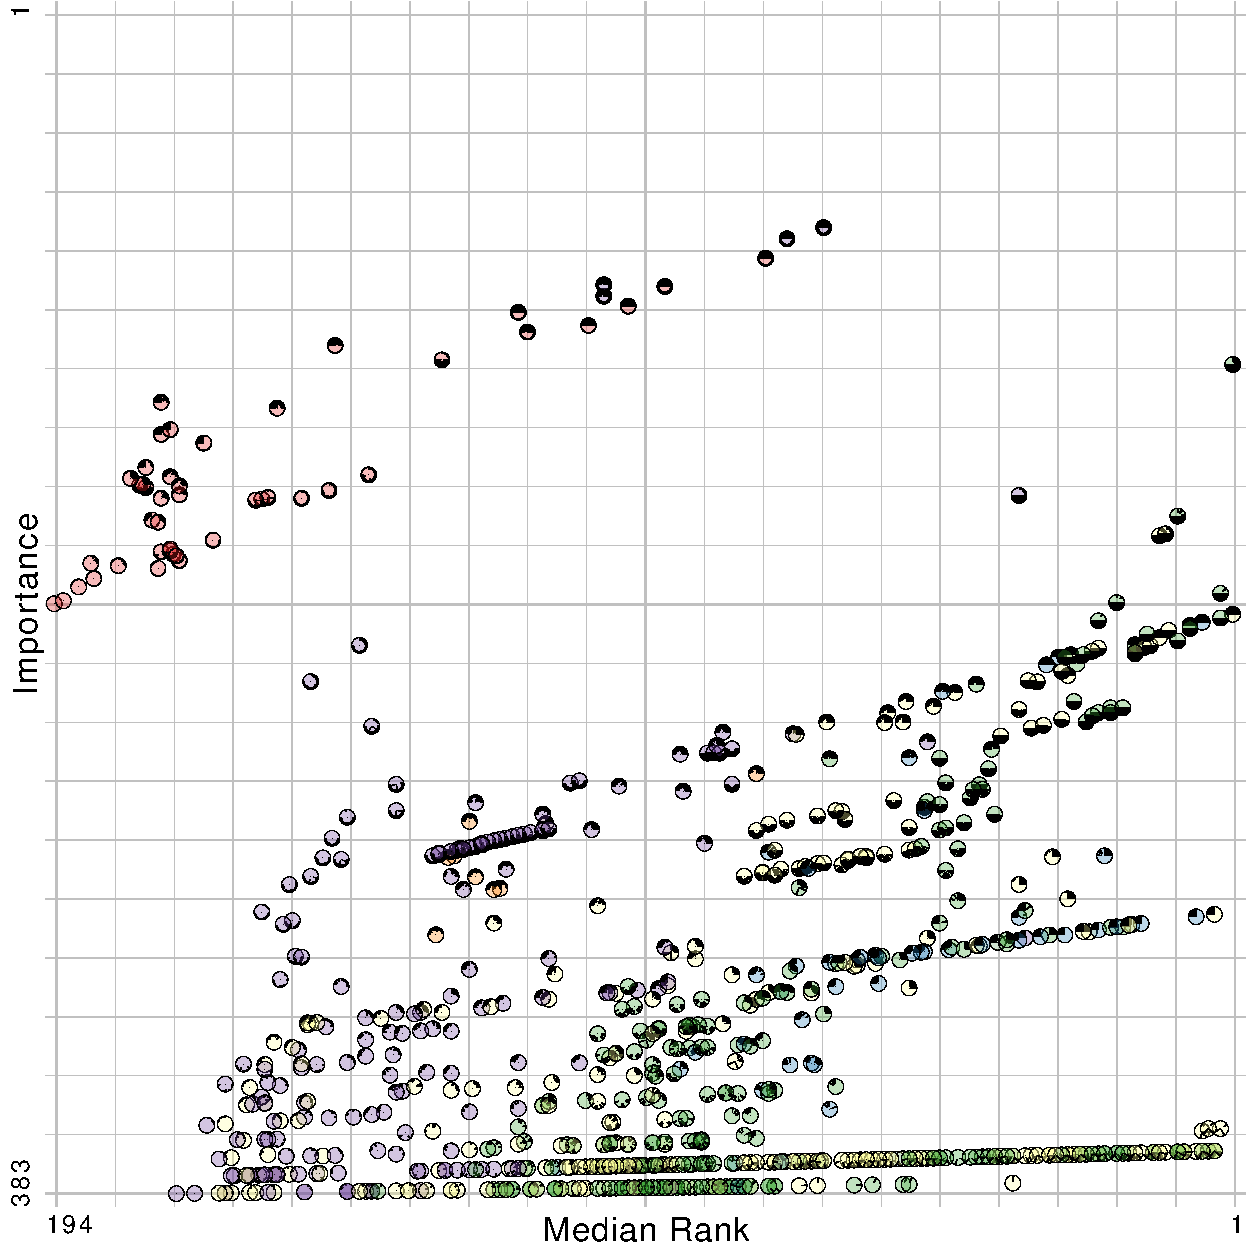
\includegraphics[width=\linewidth]{infuse/mi}
\label{subfig:mi}
\end{subfigure}%
~%
\begin{subfigure}{0.24\linewidth}
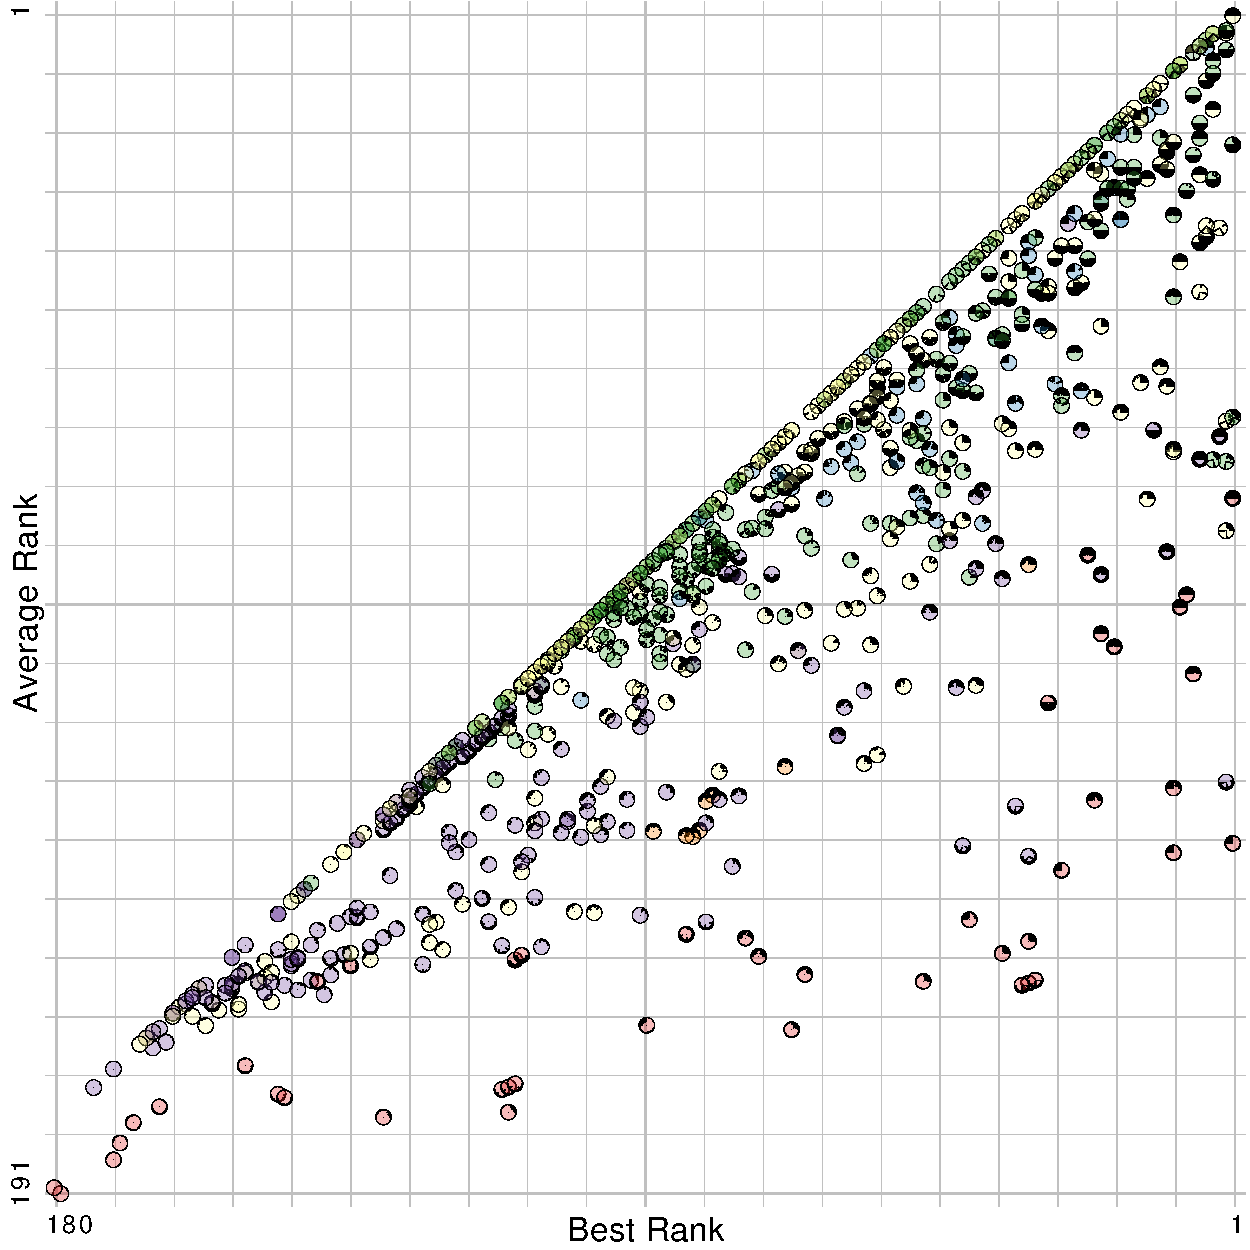
\includegraphics[width=\linewidth]{infuse/ba}
\label{subfig:ba}
\end{subfigure}%
~%
\begin{subfigure}{0.24\linewidth}
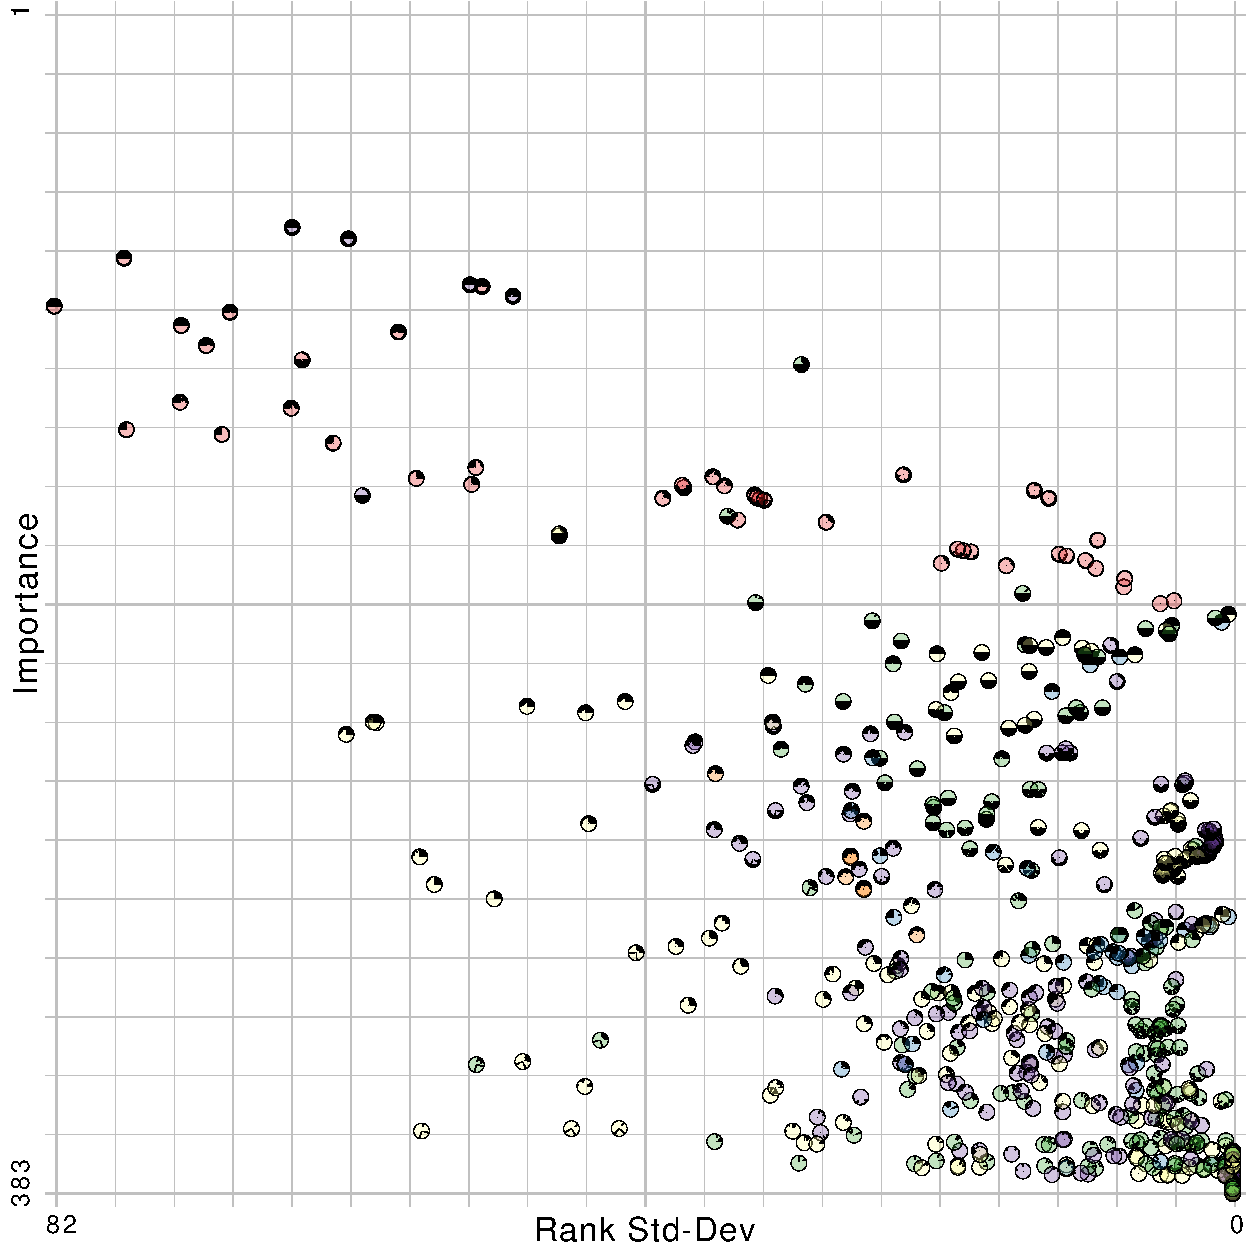
\includegraphics[width=\linewidth]{infuse/si}
\label{subfig:si}
\end{subfigure}
\caption{
Different axis combinations for the scatter-plot layout.
In \subref{subfig:ap} the average rank is plotted against the pick count.
Most of the features appear in the lower half because features are rarely picked by more than two algorithms in this example.  The bottom-right shows features that are only chosen
by two models but were ranked very high by them.
\subref{subfig:mi} shows the median rank plotted against the importance.
Notice that the plot looks similar to \subref{subfig:ap} since importance
is a combination of the axes from \subref{subfig:ap}.
The axes in \subref{subfig:ba} are best rank versus average rank.
Features can only appear below the diagonal.
The standard deviation of the ranks is plotted against the importance
in \subref{subfig:si}.
The peak to the bottom right corner consists of features that are rarely
picked and therefore have lower variance.
The peak to the top right consists of features that
are consistently high ranked.
}
\label{fig:scatter}
\end{figure*}

\subsection{Feature View}
The primary component of \infuse is the \textit{Feature View}, a zoomable visualization that displays all features as glyphs. Each glyph represents a feature from the original data set and is designed to provide the information outlined above. The main purpose of the feature view is to allow comparison between features and detection of interesting commonalities and differences in terms of how the algorithms rank them. The view allows the user to display the feature set according to two different configurable layouts: a grid layout (the default), which favors legibility, and a scatter plot layout which aims at laying out and grouping the features according to various statistics we collect from the ranks. In the following sections, we describe the design of the glyph as well as the different layouts.

% The design of the glyphs is discussed in Section~\ref{sec:glyphdesign}.
% The glyphs can be laid out in two different ways in the visualization,
% ordered by type and overall importance as described in
% Section~\ref{sec:rankedlayout}, or by positioning them
% on a scatterplot with user defined axes
% (Section~\ref{sec:scatterplotlayout}).
% By clicking on features, the user can toggle its selection.
% A group of features can be selected at once via lasso selection.

\subsubsection{Feature Glyph Design}\label{sec:glyphdesign}
% \adam{on our next phonecall, lets discuss why you call these starburst charts.  there is nothing hierarchical about this data.}
% \adam{note:  low and high ranks are used in misleading ways.  i'm putting this note to make sure we double-check to make sure we're consistent.}
As described in Section \ref{sec:motivation_healthcare}, the features are ranked by multiple feature selection algorithms and across multiple cross-validation folds.  \infuse's glyph design embeds all of this information in a circular glyph that shows all the rankings obtained from each algorithm/fold pair. As shown in Figure~\ref{fig:glyph-key}(a), the glyph is divided into equally-sized circular segments; where each segment represents one of the ranking algorithms.
For instance, in Figure \ref{fig:glyph-key}(b), since the feature was ranked by four feature selection algorithms, the circular glyph is divided into four sections. Each of these sections are then divided further into a \emph{fold slice} for each cross-validation fold. For instance, in Figure \ref{fig:glyph-key}(c), each feature selection algorithm was executed on 10 cross-validation folds, therefore there are 10 fold slices.

Within each fold slice, there is an inward-growing bar (that is, starting from the perimeter and growing towards the center) that represents the rank of the feature in a particular fold. For example, in Figure \ref{fig:glyph-key}(c), the feature is higher ranked in Fold 3 than in Fold 4 as the bar in Fold 3 stretches closer towards the center than in Fold 4. Features that are unranked, because their scores are too low to meet the minimum threshold requirement of the algorithm, are represented as empty slices with no bars. We designed fold slices with inward-growing bars on purpose to help distinguishing between slices with empty values from those with low values. During our design iterations we realized in fact that outward pointing bars would make this distinction too hard to make. Since the information of whether a features is picked up by an algorithm is crucial for its interpretation we decided to opt for this design.

%this way on purpose to have bars growing from the perimeter to the center of the circle so that folds with poor ranks can be easy detected since a fold slice has greater area closer to the perimeter.  This makes it possible to identify the basic properties of a feature selection model even when the interface is zoomed-out.



% Features are shown as inward growing starburst pie chart glyphs showing their ranking in the different models. Each pie slice represents one model. The better the rank of the feature the more the slice expands towards the center of the glyph \emph{ie.} when the feature is ranked as number one by the model the corresponding slice has the same radius as the glyph.
% If the feature is not ranked by the model the slice is not shown.
% Letting slices grow from the outside to the inside makes
% low ranks easier to read since a pie slice has a greater area at the outside.
% This enables to see low ranks and identify their model even when
% the visualization is zoomed out.
% For pie slices growing towards the outside it is difficult to
% identify the model when a rank is low.
% Consider a feature that is ranked very low in only one
% model and unranked in the other models.
% When zoomed out only a dot in the center of the glyph is visible.
% This dot could grow in any direction representing any model.
% Also, as shown in Figure~\ref{fig:glyph_design},

% Figure \ref{subfig:pie} shows an example of a glyph where the fold slices grow from the center towards the perimeter. From the figure one can see that distinguishing empty values is harder with this solution than the one we selected.

%Consider the situation where there is a lowly-ranked feature only ranked in one fold slice section.  When zoomed-out, the glyph would just appear as a circle with a dot in the center, and the user would not know which model or fold ranked the feature.

%Furthermore, it is difficult to see in which fold a feature is unranked when the surrounding models rank the feature.

Multiple glyph designs were considered and tested within \infuse.  For instance, Figure \ref{subfig:pie} shows an example of a glyph where the fold slices grow from the center towards the perimeter.
This makes it difficult to identify fold slices with poor ranks.
Consider the situation where there is a lowly-ranked feature only ranked in one fold slice section.  When zoomed-out, the glyph would just appear as a circle with a dot in the center, and the user would not know which model or fold ranked the feature.  Furthermore, it is difficult to see in which fold a feature is unranked when the surrounding models rank the feature.  Other glyph designs that were tried involve a star glyph (Figure \ref{subfig:star}) and a matrix glyph (Figure \ref{subfig:matrix}).  The star glyph was less effective as users were not afforded a reference point for the maximum ranking and the design leads to some visual artifacts (like high density in the center and lower density in the outer part).
The matrix glyph was less effective, as perceiving differences is more difficult when using luminance than length and area as we do in our final design.

%Furthermore, both of these charts were also less suited for a zoomable user interface than the chosen design.

Users can gain more details about each section and slice by hovering over the region of interest to view an informative tooltip. Furthermore, an overview key is available to remind users of the position of each model type. The background color of the glyph corresponds to the subtype of the feature and a color key can also be shown as a reference to remember the meaning of the color coding (see bottom-left corner of Figure~\ref{fig:system}).

% Pie slices are ordered by feature selection
% algorithm first and then by fold.
% This groups all results from one feature selection algorithm together
% and creates quadrants which can be used for reasoning.
% A key for those quadrants can be shown in the visualization
% and when hovering a slice with the mouse the identity of the model
% and the rank is shown in the tooltip.

% A circle with the radius of the glyph is drawn to distinguish glyphs
% from each other and defines the value bounds.


% Using colors to show ranks, for example as cell colors of a
% feature selection algorithm by fold matrix,
% is not as easy to read as the presented glyph.
% Also, normal starburst glyphs do not work very well when the
% visualization is zoomed out as the lines become thinner and harder to see.

\vspace*{1em}
\subsubsection{Ranked Layout}\label{sec:rankedlayout}
The first layout available to users is the ranked layout, which arranges glyphs by their feature type, and sorts them by their overall importance.  The name of the feature type is shown at the first position in the group, after that the features are laid out row-first in a grid-like manner, as shown in Figure \ref{fig:system}. This space-filling approach results in features that are always visible without overlaps.

Features within a group are sorted by their importance. Importance is computed as average rank with
penalized unranked features:
\[
rank_{best} = \min_{m \in M \times V, f \in F}{[rank_{m}(f)]}
\]\[
i(f) = \dfrac{1}{| M \times V |}[
2 \cdot rank_{best} \cdot
unranked_{M \times V} (f)
+ \sum_{m \in M \times V} rank_{m}(f)
]
\]
where $M$ is the set of models, $V$ is the set of cross-validation folds,
$F$ is the set of features,
$rank_{m}(f)$ is the rank of a feature $f$ in the combined model
and cross-validation fold $m$,
and $unranked_{M \times V} (f)$ is the number
of such combined models that did not choose $f$.
Assume $rank_{m}(f) = 0$ for unranked features $f$
in the combined model $m$ only when computing $i(f)$.
Note that a small value for $i(f)$ means higher importance.
The optimal value is $1$.

\subsubsection{Scatterplot Layout}\label{sec:scatterplotlayout}
The second layout available to users is the scatterplot layout, where users can select choices for both axes of the scatterplot.  The choices for axes include:

\begin{itemize}
\item the \emph{average rank} of a feature\\
(ignores unranked folds and models)
\item the \emph{pick count} of the number of combined
models\\and cross-validation folds that picked the feature
\item the \emph{importance} of a feature (defined above)
\item the \emph{best rank} of the feature
\item the \emph{median rank} of the feature\\
(ignores unranked folds and models)
\item the \emph{standard deviation} of the feature's ranks\\
(ignores unranked folds and models)
\end{itemize}

By default, the average rank is chosen for the horizontal axis and
the pick count is chosen for the vertical axis, as shown in Figure \ref{fig:usecase2}.  This combination of axes led to the most insights during the case studies.  However, if users choose to select different axes or pivot to a different layout, animation is used for the transition.  By using slow-in and slow-out animation, users are given time to anticipate the movement direction of the feature, and are able to track features during the transition easily.

% The combination of those axis contents give the most insights.
% The values of the axes are mapped from the
% minimum to the maximum value.
% The lower left corner of the scatter-plot is consistently the
% worst values of both axis and the top left corner is always the best
% values of both axis contents.

\subsubsection{Interaction}
The Feature View provides a number of interactions.
Zooming and panning enables a user to get an overview of the
displayed data and focus on the details of a small number of glyphs.  This exploration can be reset by clicking on the
``Reset View" button, or double clicking on the background. Double clicking on a feature glyph zooms in on the feature so that it fills the viewport.
In addition, a tooltip is shown when a user hovers the mouse
over a glyph. This tooltip provides information about the name, type,
and subtype of the represented feature, as well as all of the statistical
information used for the scatterplot layout. Hovering over a fold slice
in the glyph gives further information about the feature selection algorithm,
the cross-validation fold, and the feature's rank in question.  In order to select features for interactive model building
(see Section~\ref{sec:imb}) the user can click on glyphs to toggle
the selection or use a lasso gesture to select a group of features.
As mentioned in the previous section, users can change the
layout of the glyphs with the buttons below the Feature View.

\subsection{List View}
A simple yet important view of features is the List View, which provides a sorted list of all features, useful for selecting features by name.  Each list item contains the name of the features along with its glyph.  The selection of a feature can be toggled in the list by clicking its list item.  As the selection of features is linked between views, this sorted and labeled view supports users finding particular features of interest and highlighting them in the complementary views.

The list view can be sorted in a few different ways. By default, features are first sorted by
the type of the feature, then by its subtype, and finally by its name.  Users can also sort the list by selection, which means currently selected features are displayed at the top and the unselected features appear after them.  Within these groups, the features are then sorted by their importance.

In addition to sorting, a user can filter the list view via the search box on
the top.
Search terms are separated by white-spaces and the list view
shows all features that contain all search terms in the name, type, or
sub-type.
The results are ranked by the sum of the inverse positions
of the search terms within the feature description.
This favors terms occurring at the beginning of the feature's name
and terms that occur multiple times in one feature description
(see the top right panel of Figure~\ref{fig:system} for an example query).

\begin{figure}[t]
\centering
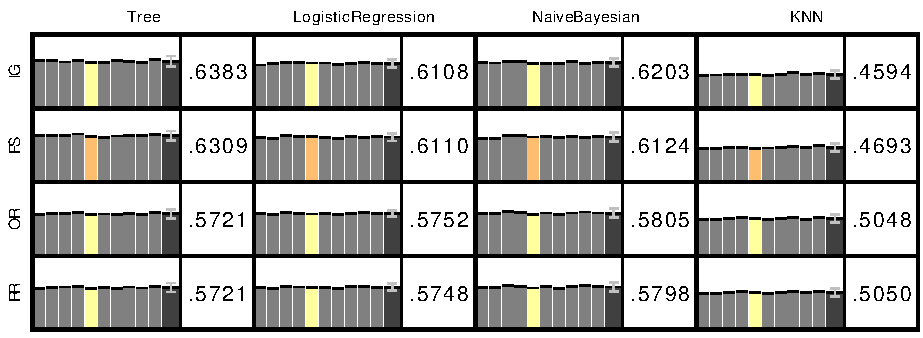
\includegraphics[width=0.8\linewidth]{infuse/classifier}
\caption{The Classifier View displays the results of the classification algorithms for all models.
Rows represent feature selection algorithms and columns represent classification algorithms.
A more detailed description of the cells can be
seen in Figure~\ref{fig:classifier-cell}.
The currently selected model is highlighted in orange, and the results for the same fold in different
feature selection algorithms are highlighted in yellow.  When users select a model, the features that make up the model are highlighted in the Feature and List views.
}
\label{fig:classifier}
\end{figure}

\begin{figure}[b]
\centering
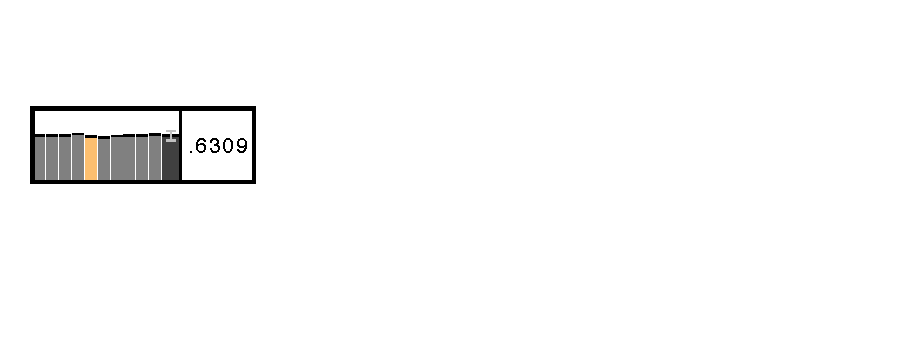
\includegraphics[width=0.5\linewidth]{infuse/classifier-cell}
\caption{
Each cell in the Classifier View represents the scores of a particular model by a particular classifier.
On the left, there is a bar for each of the validation folds.  The height of each bar corresponds to the AUC score for each fold.  Immediately to the right of the fold bars, the thicker and darker bar and its height represents the average value across all folds.  This bar also features an error bar depicting the standard deviation across the folds.  Finally, to the right of the bars, there is a numerical representation of the average AUC score.}
\label{fig:classifier-cell}
\end{figure}

\subsection{Classifier View}

The Feature View and the List View both focus on supporting users to interpret the rankings of features across multiple predictive models.  However, it is also important for users to understand the quality of each model in predicting the appropriate outcome.  The Classifier View, shown in the bottom-right panel of \infuse, is where the quality of each the predictive models can be analyzed.

Typically, predictive models are evaluated using classification algorithms which provide an AUC score (area under ROC curve,
the sensitivity as function of the false positive rate).  Perfect models will have an AUC score of 1, whereas random guessing will have an AUC score of 0.5.  The Classifier View was designed to show AUC scores for each model and fold.

As illustrated in Figure \ref{fig:classifier}, each row of the Classifier View represents the predictive model that resulted from each feature selection algorithm.  Each column represents a classification algorithm.  Multiple classifiers are used because there are a variety of techniques to evaluate models, and in order to avoid biases, \infuse provides the ability to compare the output from multiple classifiers.

Each cell, as shown in Figure \ref{fig:classifier-cell}, has several components.  On the left, there is a bar for each of the validation folds.  The height of each bar corresponds to the AUC score for each fold.  There is also a slightly thicker and darker bar immediately to the right of the fold bars, and its height represents the average value across all folds.  This bar also features an error bar depicting the standard deviation across the folds.  Finally, to the right of the bars, there is a numerical representation of the average AUC score.  As this information is important for predictive modelers to reason about the quality of models, these values are given visual prominence. The bars, however, can be used to also reason about the quality across all folds.

% A matrix showing feature selection algorithms as rows and
% classification algorithms as columns shows those values.
% Each cell is divided into two parts.
% The first part splits the averaged result for one feature selection
% algorithm into the results of the underlying folds.
% The areas under curve for all folds are shown as bar charts.
% The average area under curve for this
% pair of feature selection and classification algorithm is shown
% as slightly thicker and darker bar on the right end of the bar chart.
% An error bar depicts the five times amplified standard deviation
% over the folds.
% The second part shows the average area under curve as actual number.
% This is important for users to be able to directly reason about the values.

Rows are sorted by the average AUC scores across all classification algorithms, so more accurate predictive models appear at the top of this view.  Users can interact with this view in several ways.  Clicking on a fold bar selects all features that were a part of this model and highlights them in the List and Feature views.  The selected fold bar is highlighted in orange, and other scores this fold received by the other classifiers are highlighted in yellow so that they can easily be compared (as shown in Figure~\ref{fig:classifier}.)

\begin{figure}[ht]
\centering
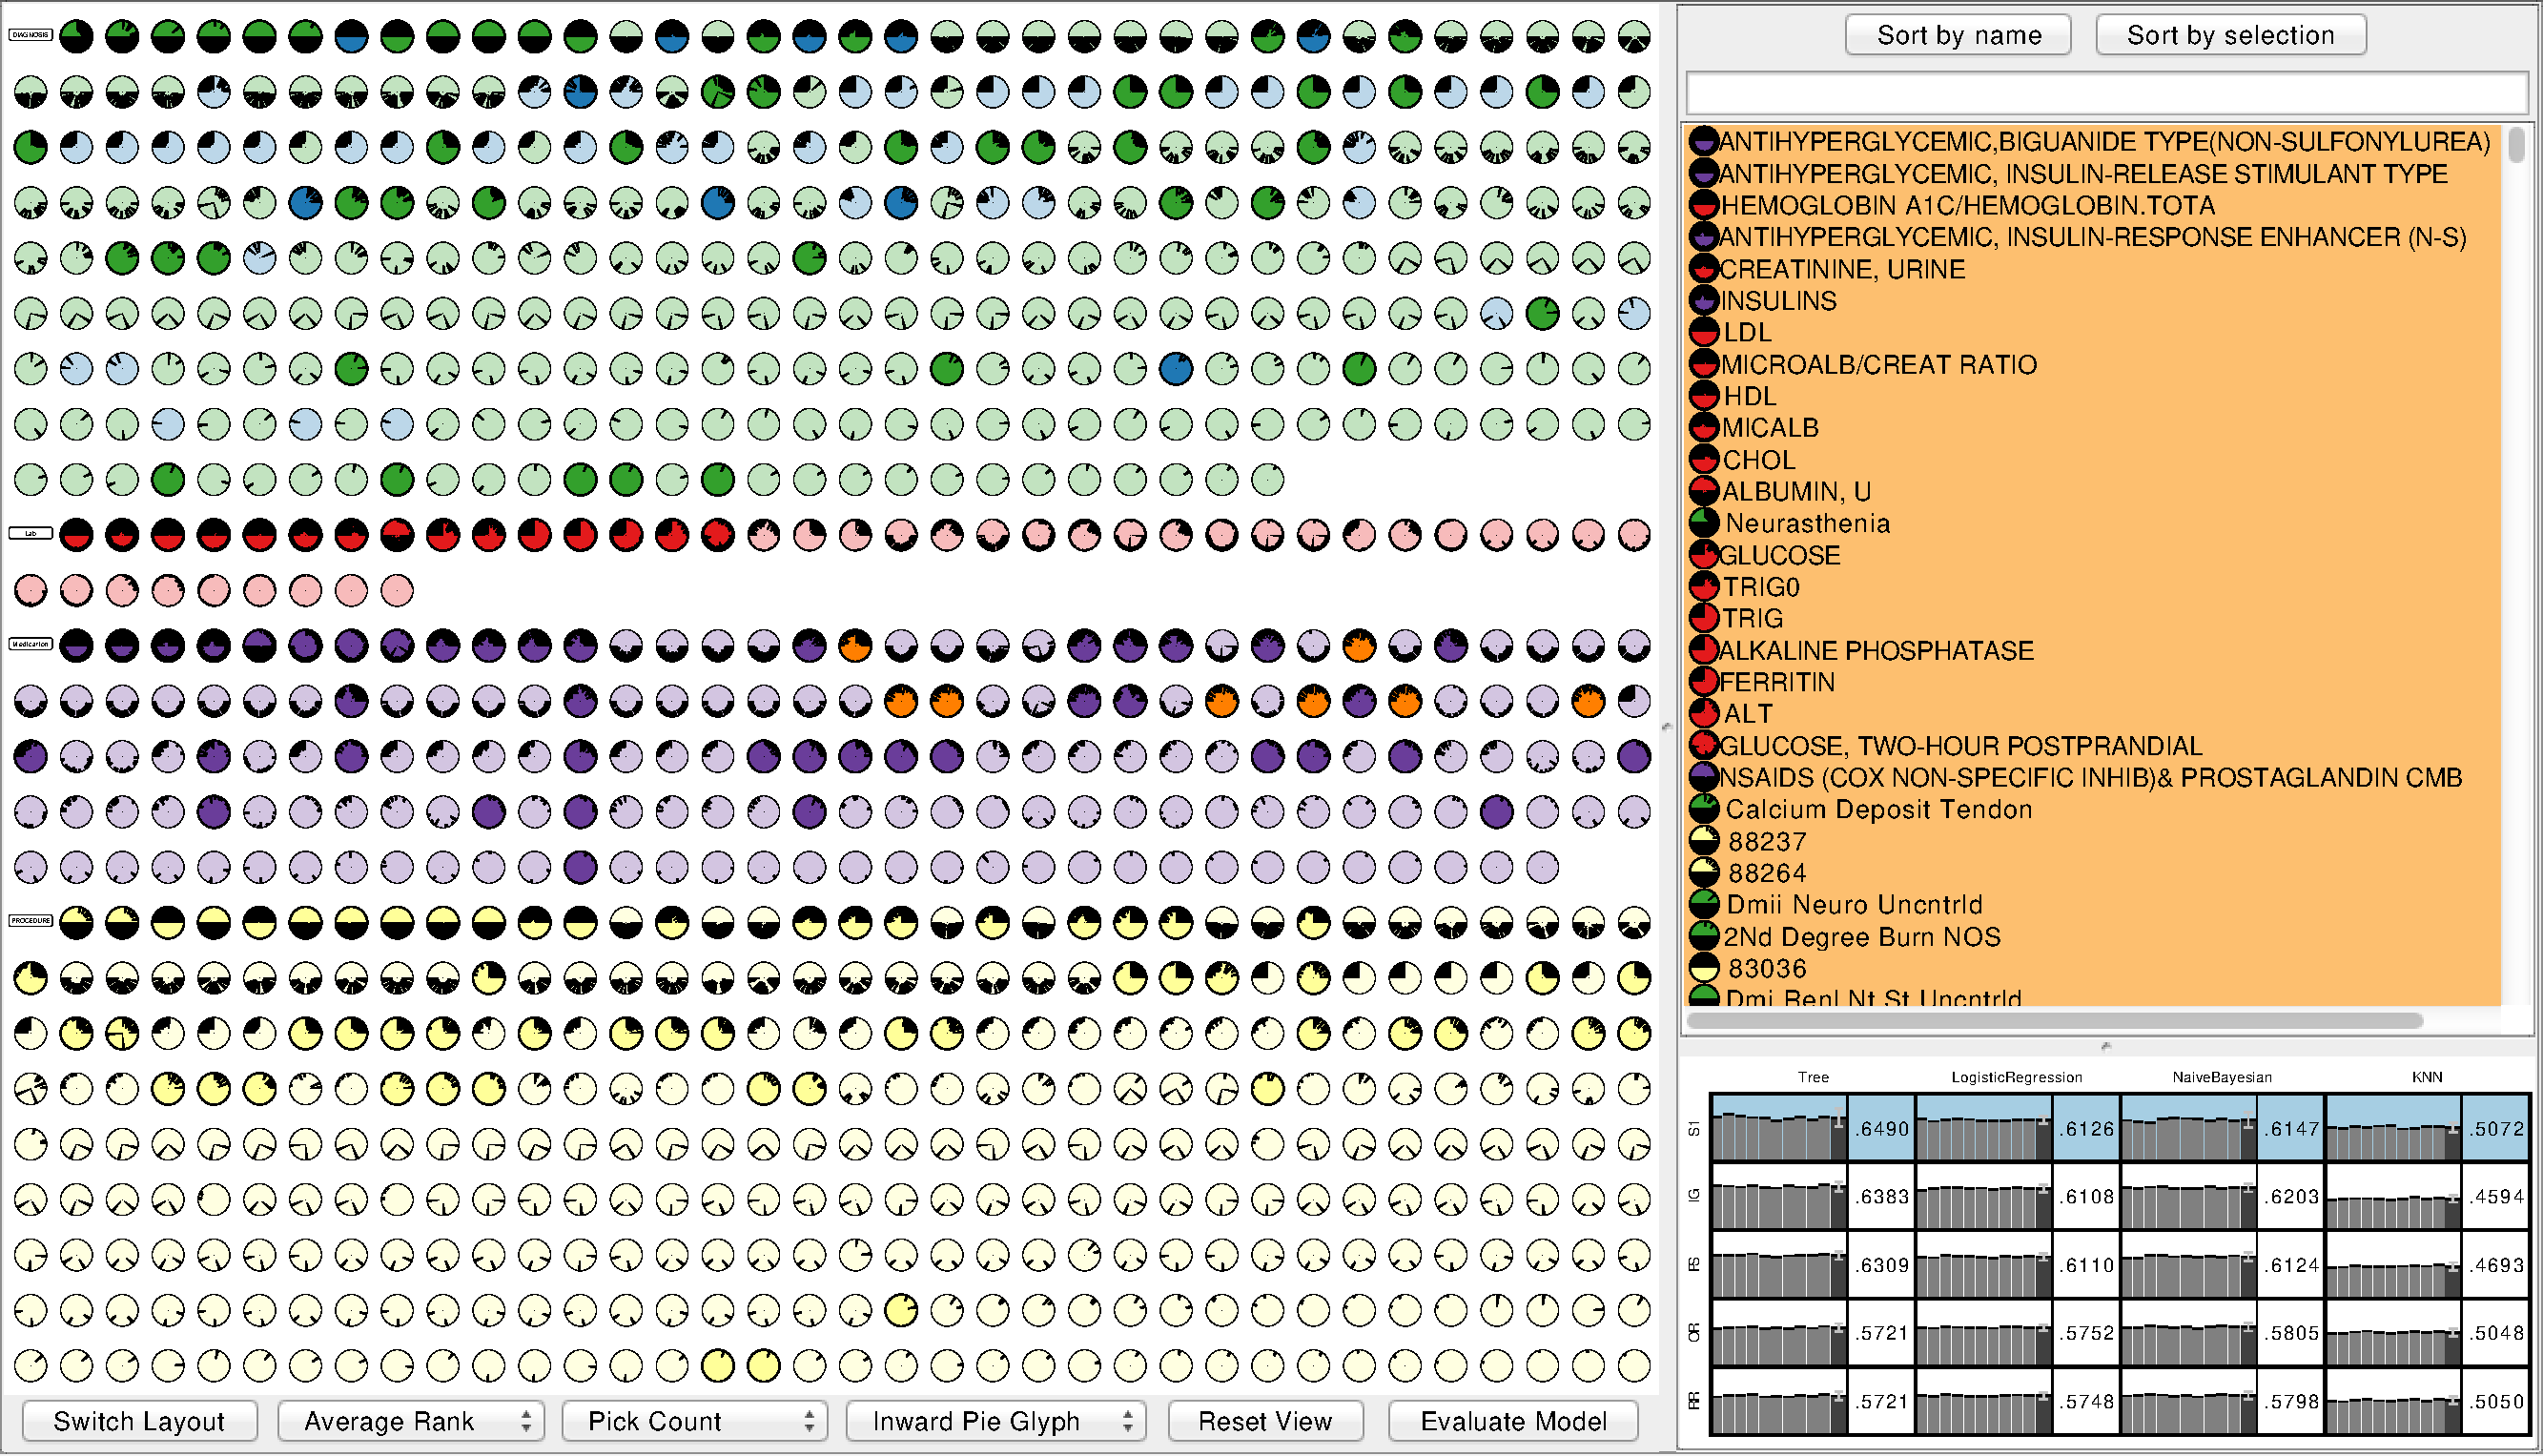
\includegraphics[width=\linewidth]{infuse/selection}
\caption{
\infuse's Interactive Model Builder allows users to select sets of features and measure its quality.
Selected feature glyphs are highlighted by saturating their color.  The List View is sorted to show the selected features by their importance.  After a user has made their selections, they can evaluate their model by clicking the ``Evaluate Model" button.  This adds a new blue row to the the Classifier View, showing the results of the evaluation for the user-defined model.
}
\label{fig:selection}
\end{figure}

\subsection{Interactive Model Builder}
\label{sec:imb}

One of the most important aspects of \infuse is that in addition to allowing the comparison of models, it also enables the creation of new models based on insights.
Users can select features for model building in a variety of ways.  They can select all of the features from existing models by clicking on a model in the Classifier View.  This will highlight and select all of the features that were used in the model.  Users can then augment these lists, or start from an empty set, by selecting individual features when clicking on them in the Feature or List view.  In order to select multiple features, a lasso selection technique is available in the Ranked and Scatterplot layouts.

After a feature set has been collected, \infuse can automatically evaluate the predictive performance of the user-defined model. By clicking the ``Evaluate Model" button,
%(\adam{Would be better named as "Evaluate Selected Model" but may not be worth doing new screenshots})
the new model is scored across all cross-validation folds and classifiers, and the results are added in the Classifier panel as a new blue row.  In the example in Figure~\ref{fig:selection}, the user-defined model out-performed the automated models and it is ranked at the top of the Classifier View.
Note that the user created model does not appear in the glyph.
This is due to the fact that the user does not need to rank the
features in order to obtain a classification result and that the feature
set is equal for all cross-validation folds.

% In every part of the system, features can be selected.
% Entire groups of features can be selected via clicking on
% a model in the classifier view or by using lasso selection in
% the feature view.
% The selection of single features can be changed by clicking in
% either the feature or list view.
% The set of selected features can eventually be used
% to create a new model.
% By clicking on the rightmost button at the bottom
% the area under curve values for the new model are computed
% and a new row is inserted at the correct position in the classifier view
% (see Figure~\ref{fig:selection}).
% This is helpful for an expert to verify whether a manually created set of
% features performs better than the automatically created sets.

% !TEX root = ../featureselection.tex

\section{Case Study}
Throughout our paper, we have used a running example of a team
of clinical researchers using predictive modeling to
classify patients at high risk of developing diabetes.
In this section, we describe how \infuse has led to a variety
of insights when exploring the features of the models.

\begin{figure*}[ht]
\centering
\resizebox{0.9\linewidth}{!}{%
\begin{tikzpicture}
\newcommand*{\imgwidth}{3.7cm}
\newcommand*{\boxsize}{0.437cm}
\newcommand*{\boxpos}{(.295, -.18)}
\newcommand*{\rightimagepos}{(4.8, 0)}
\newcommand*{\leftimagepos}{(0, 0)}
\node[inner sep=0pt] at \leftimagepos
    {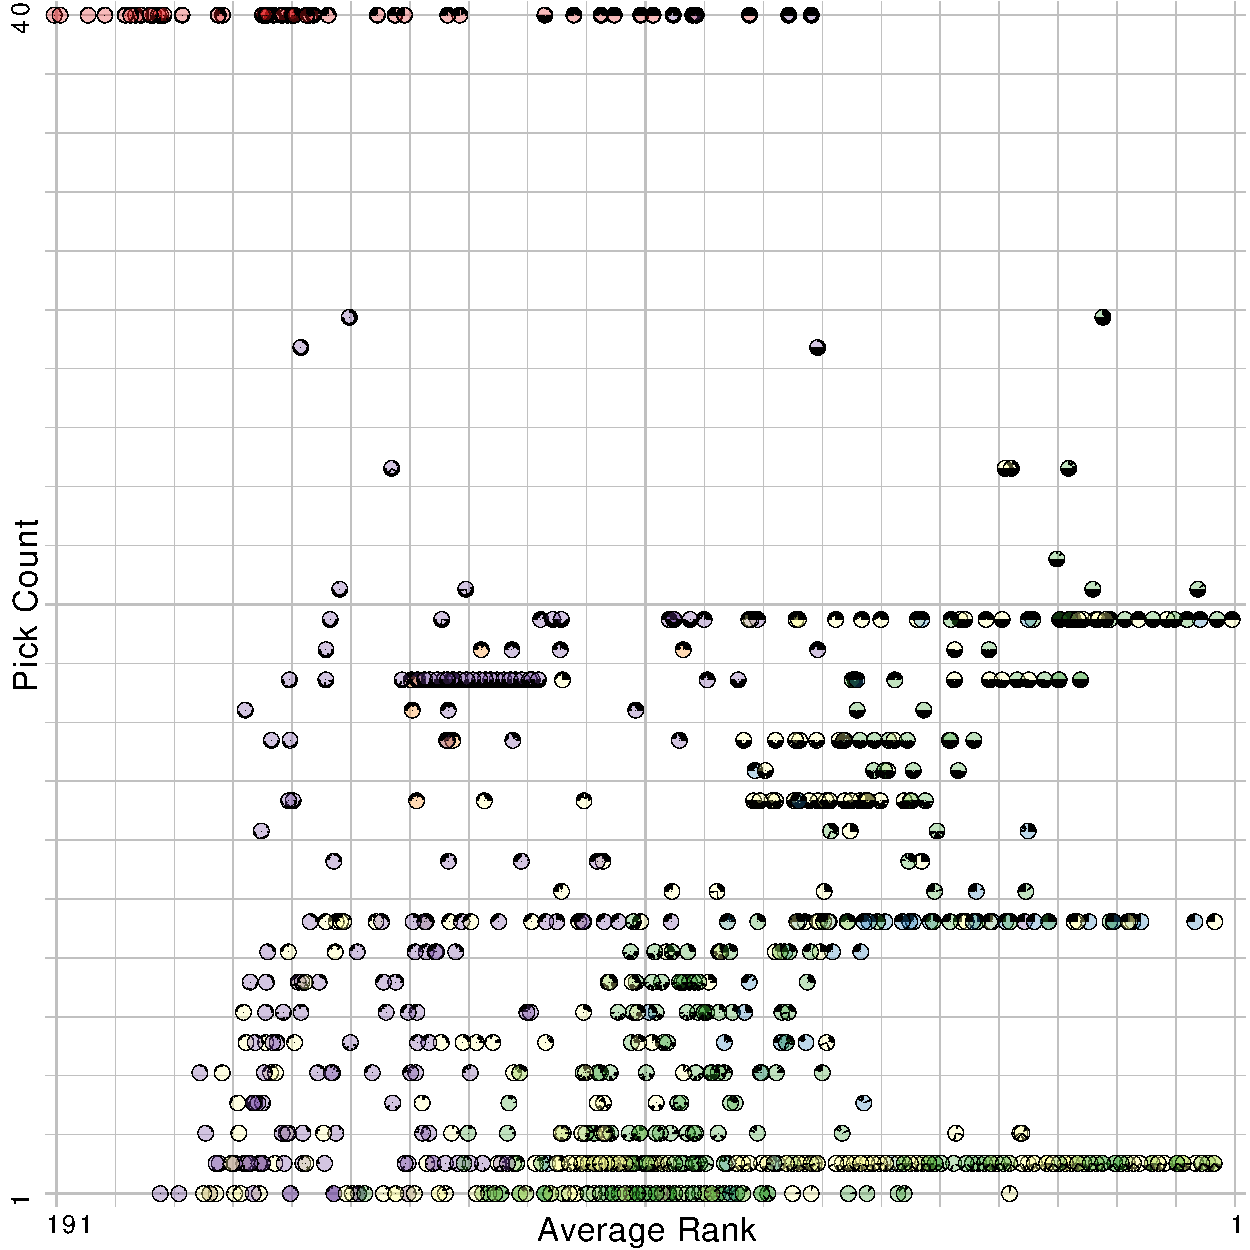
\includegraphics[width=\imgwidth]{infuse/ap}};
\node[inner sep=0pt] at \leftimagepos
    {\phantom{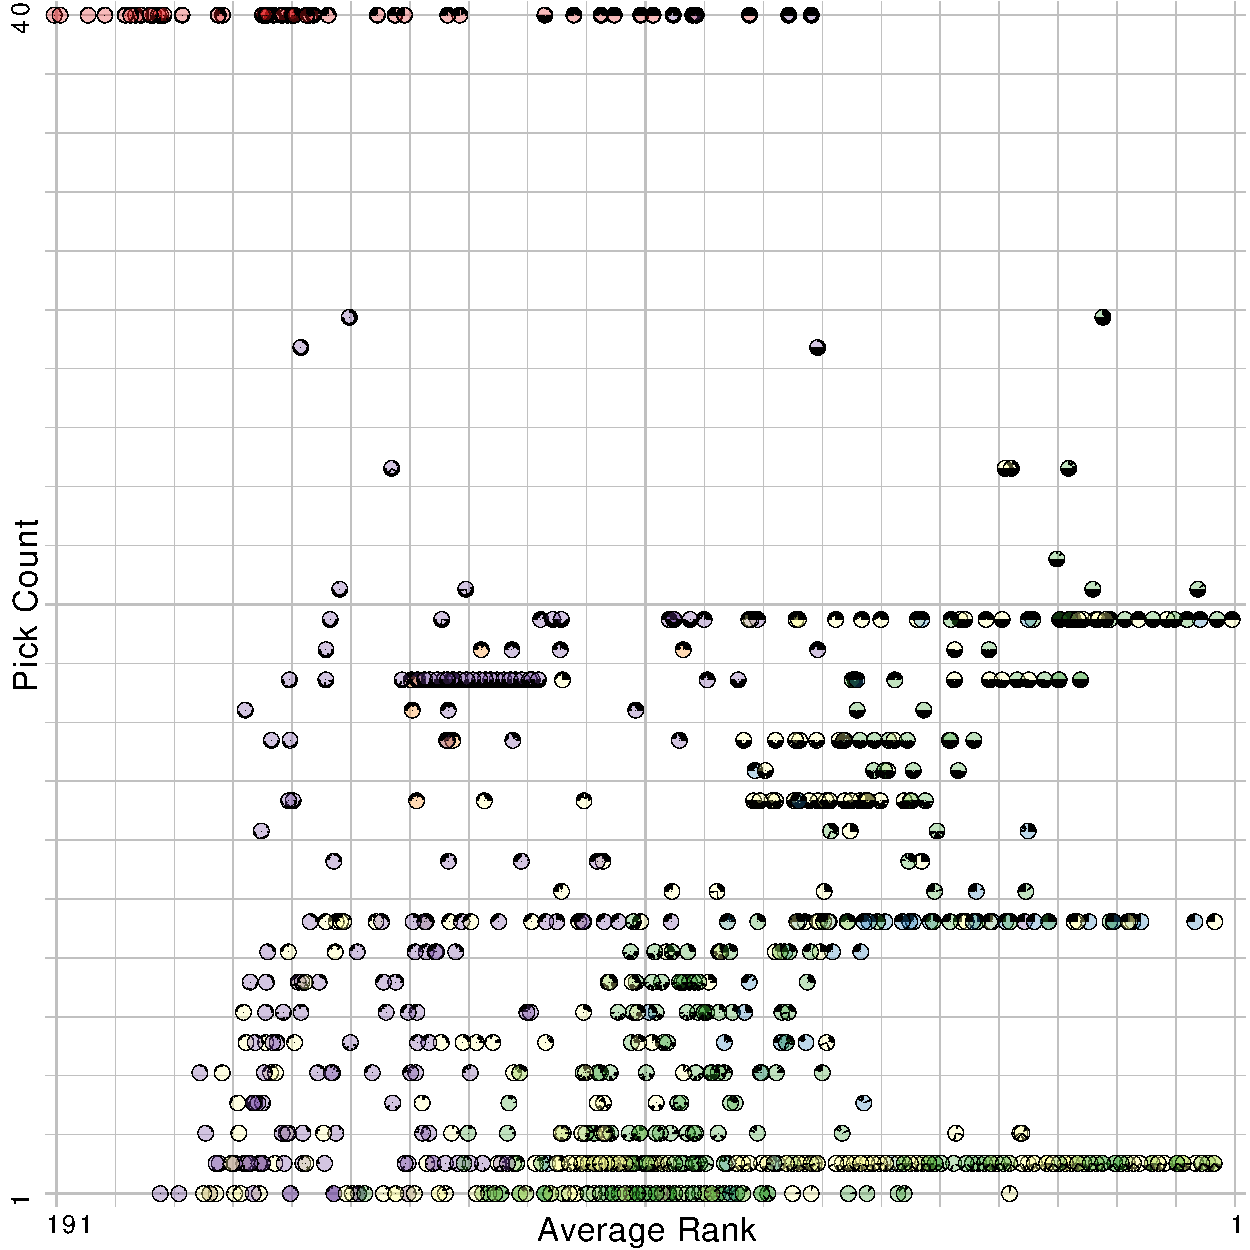
\includegraphics[width=\imgwidth]{infuse/ap}}};
\node[inner sep=2.5pt,very thick, text height=\boxsize] (zoom)
at \boxpos
    {\hspace*{\boxsize}};
\node[inner sep=-0.05pt] (lasso) at \rightimagepos
    {\phantom{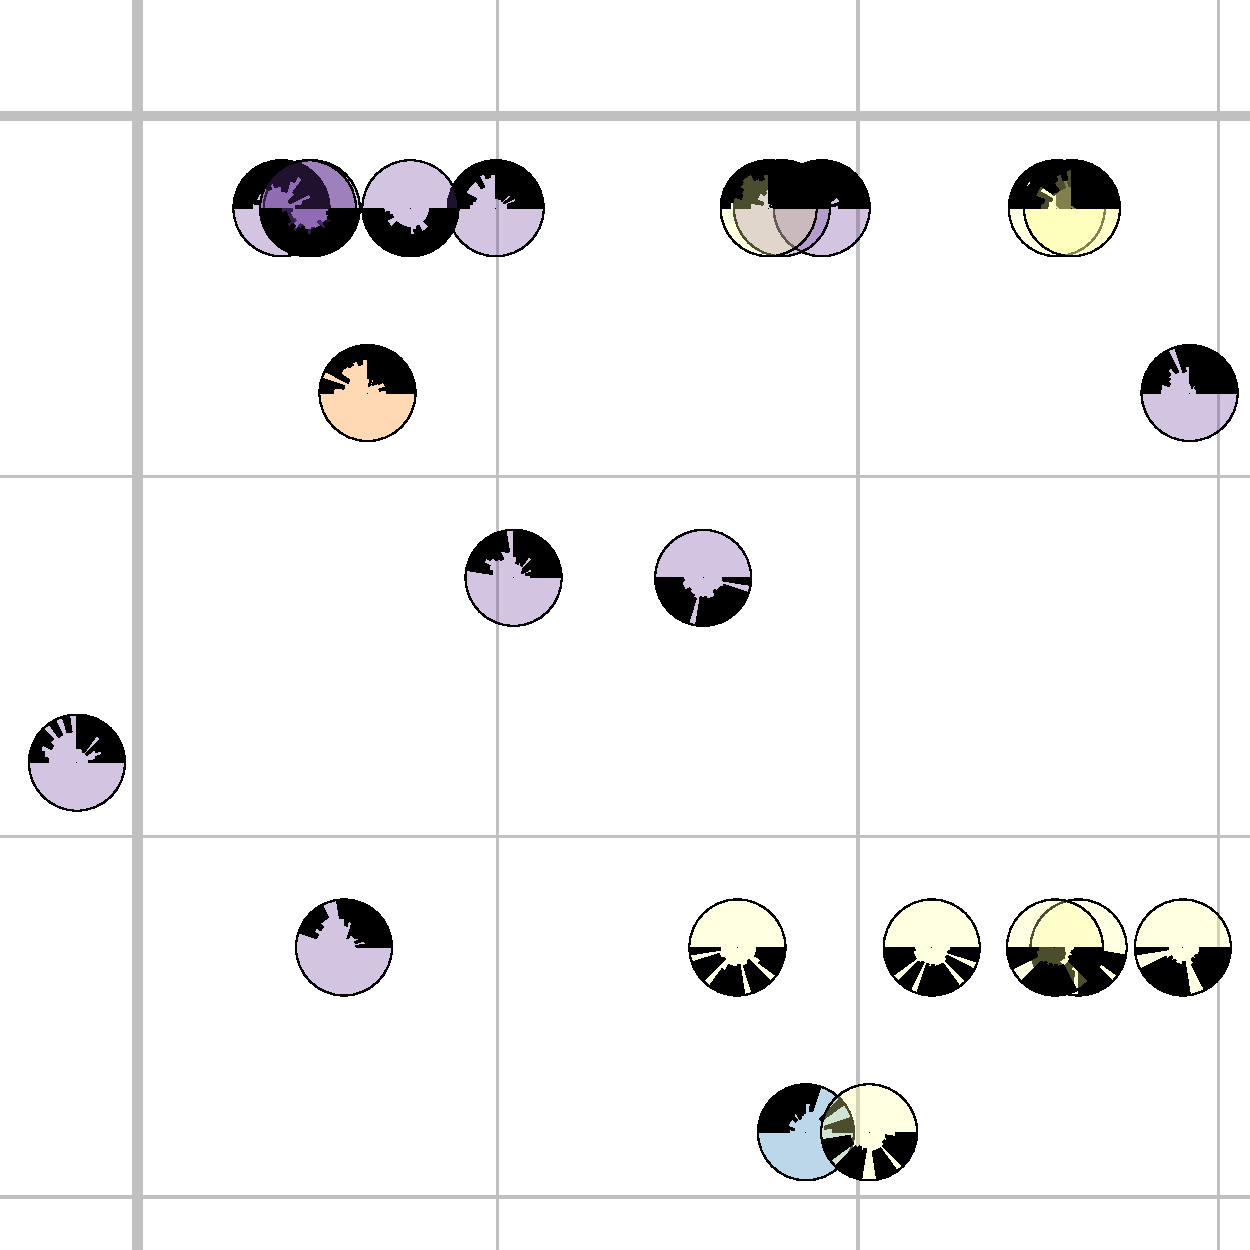
\includegraphics[width=\imgwidth]{infuse/lasso}}};
\draw (zoom.north west) -- (lasso.north west);
\draw (zoom.south west) -- (lasso.south west);
\draw (zoom.north east) -- (lasso.north east);
\draw (zoom.south east) -- (lasso.south east);
\node[very thick, draw=red!90, text height=\boxsize]
at \boxpos {\hspace*{\boxsize}};
\node[inner sep=0pt, very thick] at \rightimagepos
    {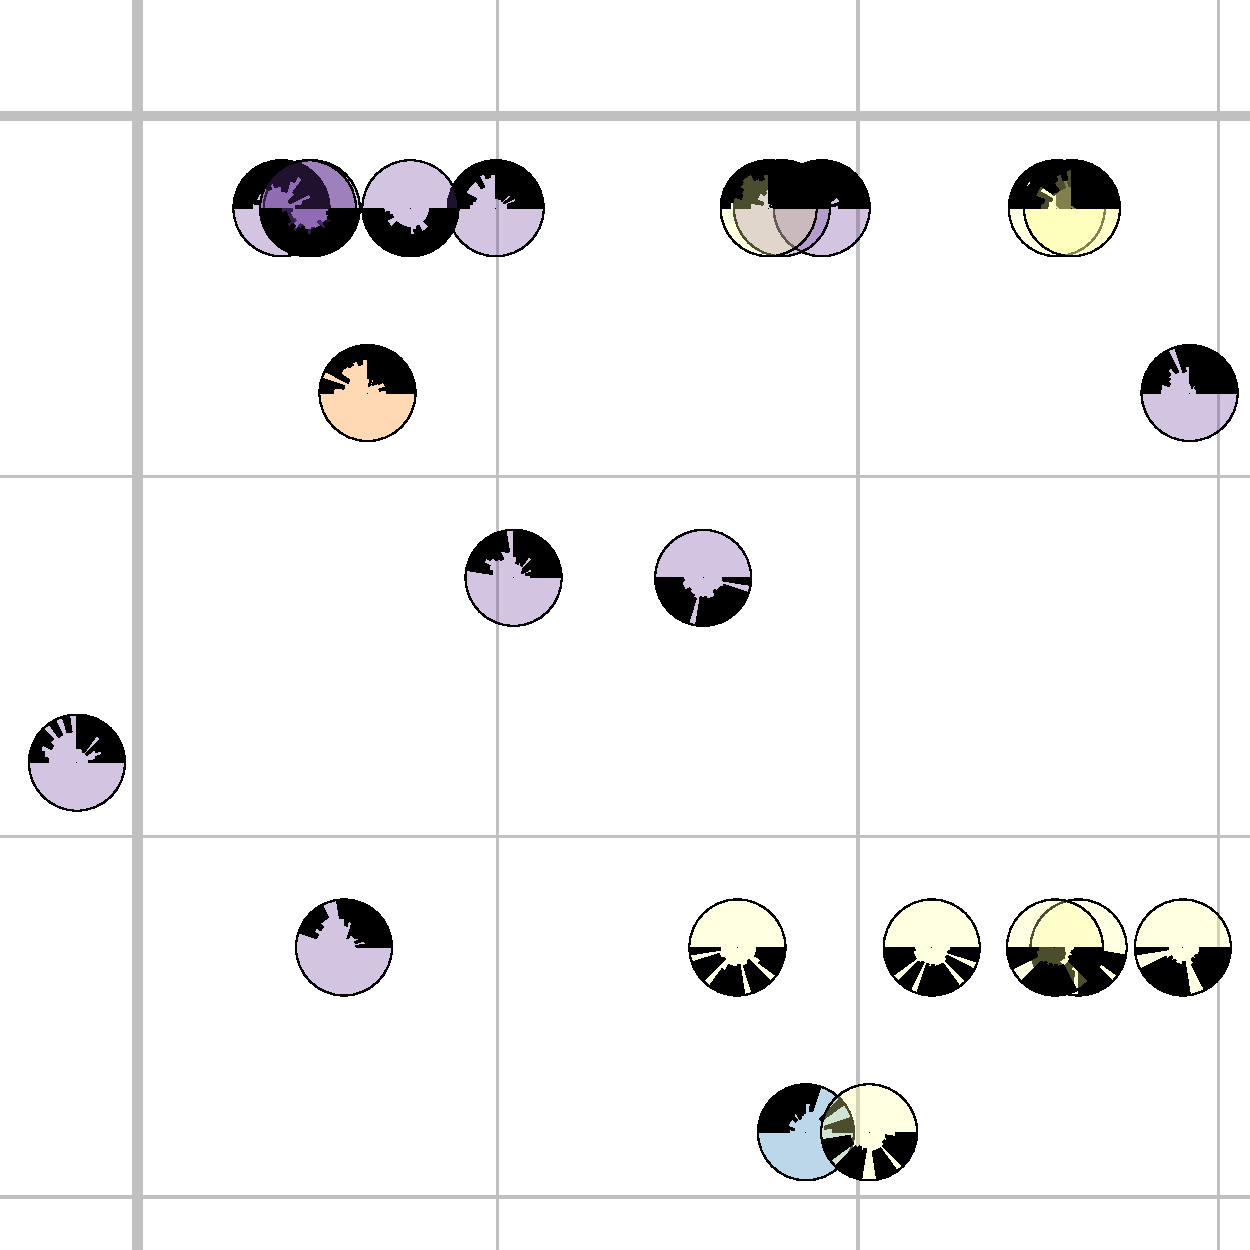
\includegraphics[width=\imgwidth]{infuse/lasso}};
\node[inner sep=0pt, very thick, draw=red!90] at \rightimagepos
    {\phantom{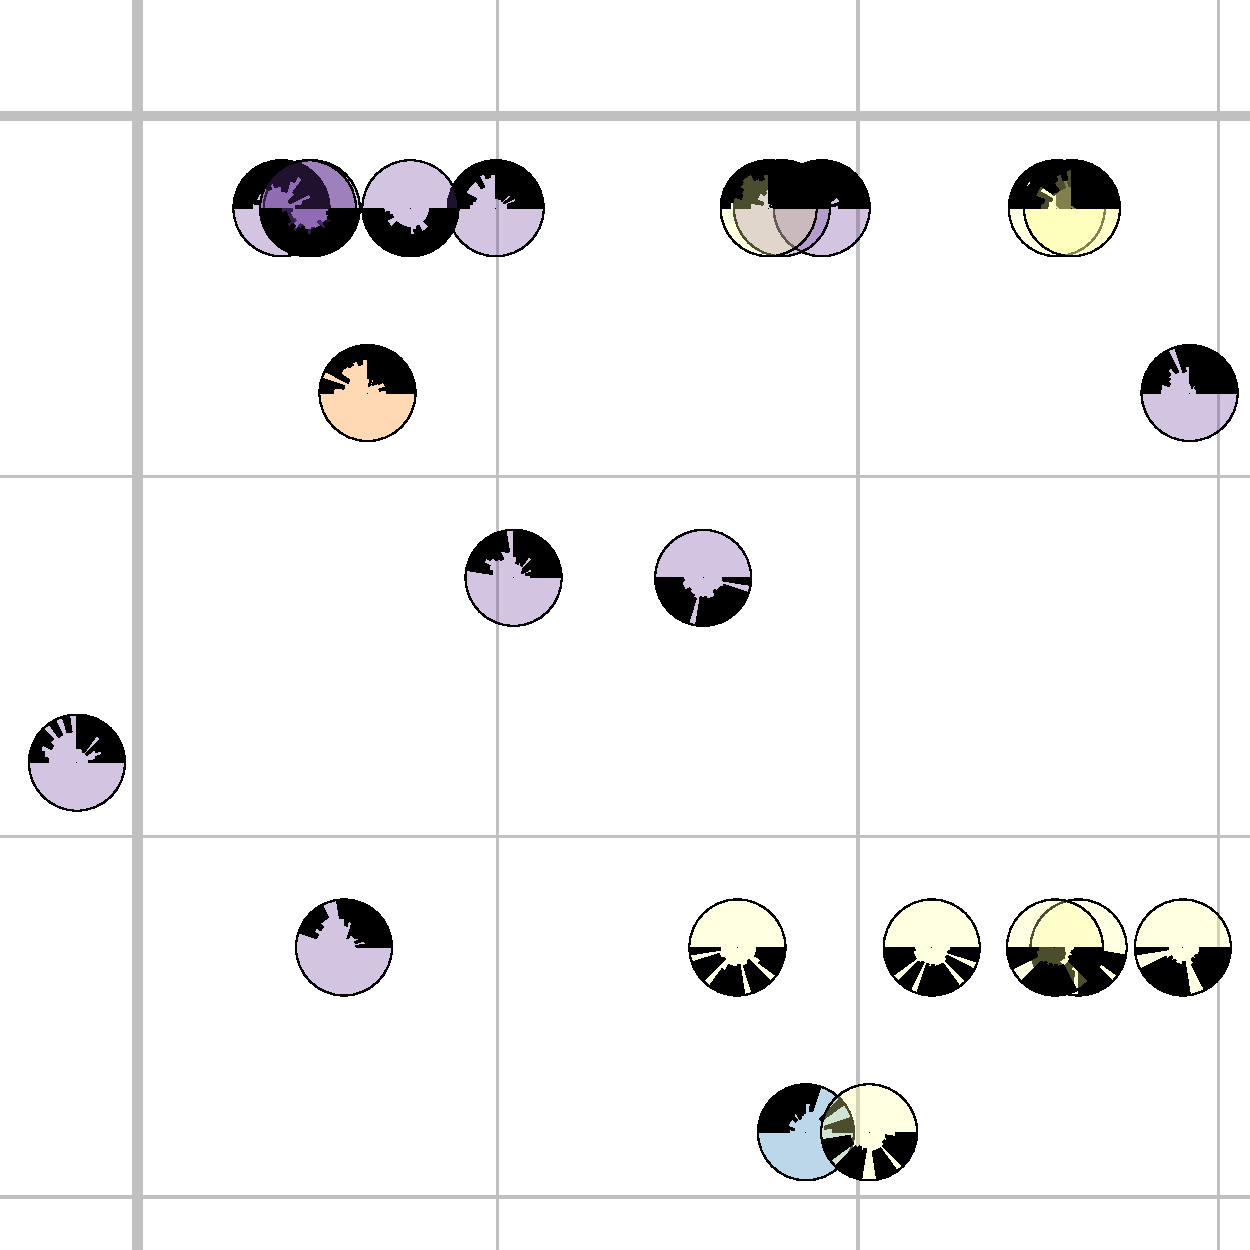
\includegraphics[width=\imgwidth]{infuse/lasso}}};
\end{tikzpicture}%
}
\caption[The scatter-plot view allows users to compare multiple types of rankings.]{
The scatter-plot view allows users to compare multiple types of rankings.  In the case study, users became curious of the medication features that were chosen by only half of the models.  When reviewing these medications with domain experts, it became clear that features picked by the upper-half algorithms were as clinically significant as those picked by the bottom-half.  This indicates that merging results from feature selection algorithms makes sense for this predictive model.
}
\label{fig:usecase2}
\end{figure*}

\subsection{Insight 1: Data issues}
When the clinical researchers learned of \infuse's capabilities
to compare multiple feature selection algorithms, they decided to
expand their pipeline's feature selection algorithms from 2 to 4.
The team has used Information Gain and Fisher Score extensively
in prior work, and typically uses these same techniques due
to their familiarity and past success.
Nonetheless, the diabetes data set introduced in Section \ref{sec:running_example} was new to them, and they were unsure which techniques would be the most appropriate. So, they asked their technologists to implement two new techniques: Odds Ratio and Relative Risk.

After all four algorithms were available, they executed their modeling pipeline
using \textit{PARAMO} \cite{paramo} and connected the results to \infuse.
Instantly, the team was surprised at the patterns that the visualization made evident.
The visualization indicated that there seemed to be little agreement between their two
old algorithms, and their two new algorithms for the best features.
The glyphs clearly indicated that many of the features were
highly ranked by two of the four feature selection algorithms,
and unranked by the other two, resulting in glyphs resembling alternating half-circles,
as shown in Figure~\ref{fig:usecase1}.
The team was quick to note that the resulting accuracy across
all four models were not significantly different,
so this non-overlap would have probably gone unnoticed if the
team just looked at resulting predictive scores at the
end of the pipeline as they typically do.

As \infuse gave them the opportunity to
examine multiple algorithms at the feature-level, they were curious as
to why this trend of non-overlapping feature rankings occurred.
They investigated the scores associated with each feature rank
and noticed that many of the features had scores
of $\infty$ from the Relative Risk algorithm.
It turned out there was a bug within the Relative Risk implementation where a
divide by zero error could happen if a feature did not occur
in any of the control patients.  After fixing this bug, they noticed that much of the non-overlap still was evident.  Looking more closely at the algorithms provided a
reason why the two new algorithms behave very differently:  they realized that both of the new algorithms only look at the presence and absence of the feature between the case and controls,
and do not pay attention to the feature values in any other way (e.g. distribution of values).
This is in contrast to the Fisher Score and Information Gain algorithms that take
the actual feature values into account.  This means that for features that are present in both case
and control groups in the same proportion, there is no discrimination value.

One of the team members mentioned, ``Each feature selection algorithm captures different types of information.  \infuse allows you to see what the effect of that information is being captured and gives you insight into the robustness of your predictive model."

As different algorithms will make sense for different purposes depending on the dataset and goals, \infuse provides an ability to inspect the features and determine
which algorithms produce ranked sets of domain-relevant features.

\subsection{Insight 2: Clinically relevant features}
After the data issues were solved, the researchers began investigating
the content of the predictive features.
Using the scatterplot view,
they inspected all of the medications that were ranked by all
feature selection algorithms and folds and found that they
were \textit{antihyperglycemic} medications, which are common treatments to lower the blood sugar of diabetes patients, and made clinical sense to be ranked high.

However, looking towards the center of the scatterplot,
where the features are only ranked by half of the algorithms and folds,
the researchers noticed a cluster of medications that
had half-circle patterns like those described above. This region is highlighted in Figure~\ref{fig:usecase2}. By mouse-hovering these features to read their names, it became clear that those ranked high by the upper-half of the circle (Information Gain and Fisher Score) were as clinically relevant and similar as those ranked by the bottom-half algorithms (Relative Risk and Odds Ratio). This provided feedback that in predictive modeling it is not safe to assume that one single feature selection algorithm is able to detect all possible interesting features and also that having a system like \infuse allows them to build a much richer picture of what kind of feature sets may lead to effective modeling. Without such a tool they would be restricted at evaluating one single algorithm at a time or, at best, restricting the comparison to a small number of features.

%it's not just certain feature selection algorithms that do not a better job overall, but instead might led themselves to finding certain features of various types -- all of which might strengthen the model.

After interacting with the system one of the team members said, ``\textit{If you just use one feature selection algorithm, you're only getting certain types of features. \infuse gives you a guide to what you might be missing. Using a combination type approach [with the Interactive Model Builder] will lead to stronger predictive models.}"

The clinical team is now going to re-think their strategy about how they
build predictive models and may consider using features by merging top
ranked features from different types of feature selection algorithms.
The researchers are convinced that by merging features, in addition
to the interactive model building capability, their predictive models will be improved.

\begin{figure}[t]
\centering
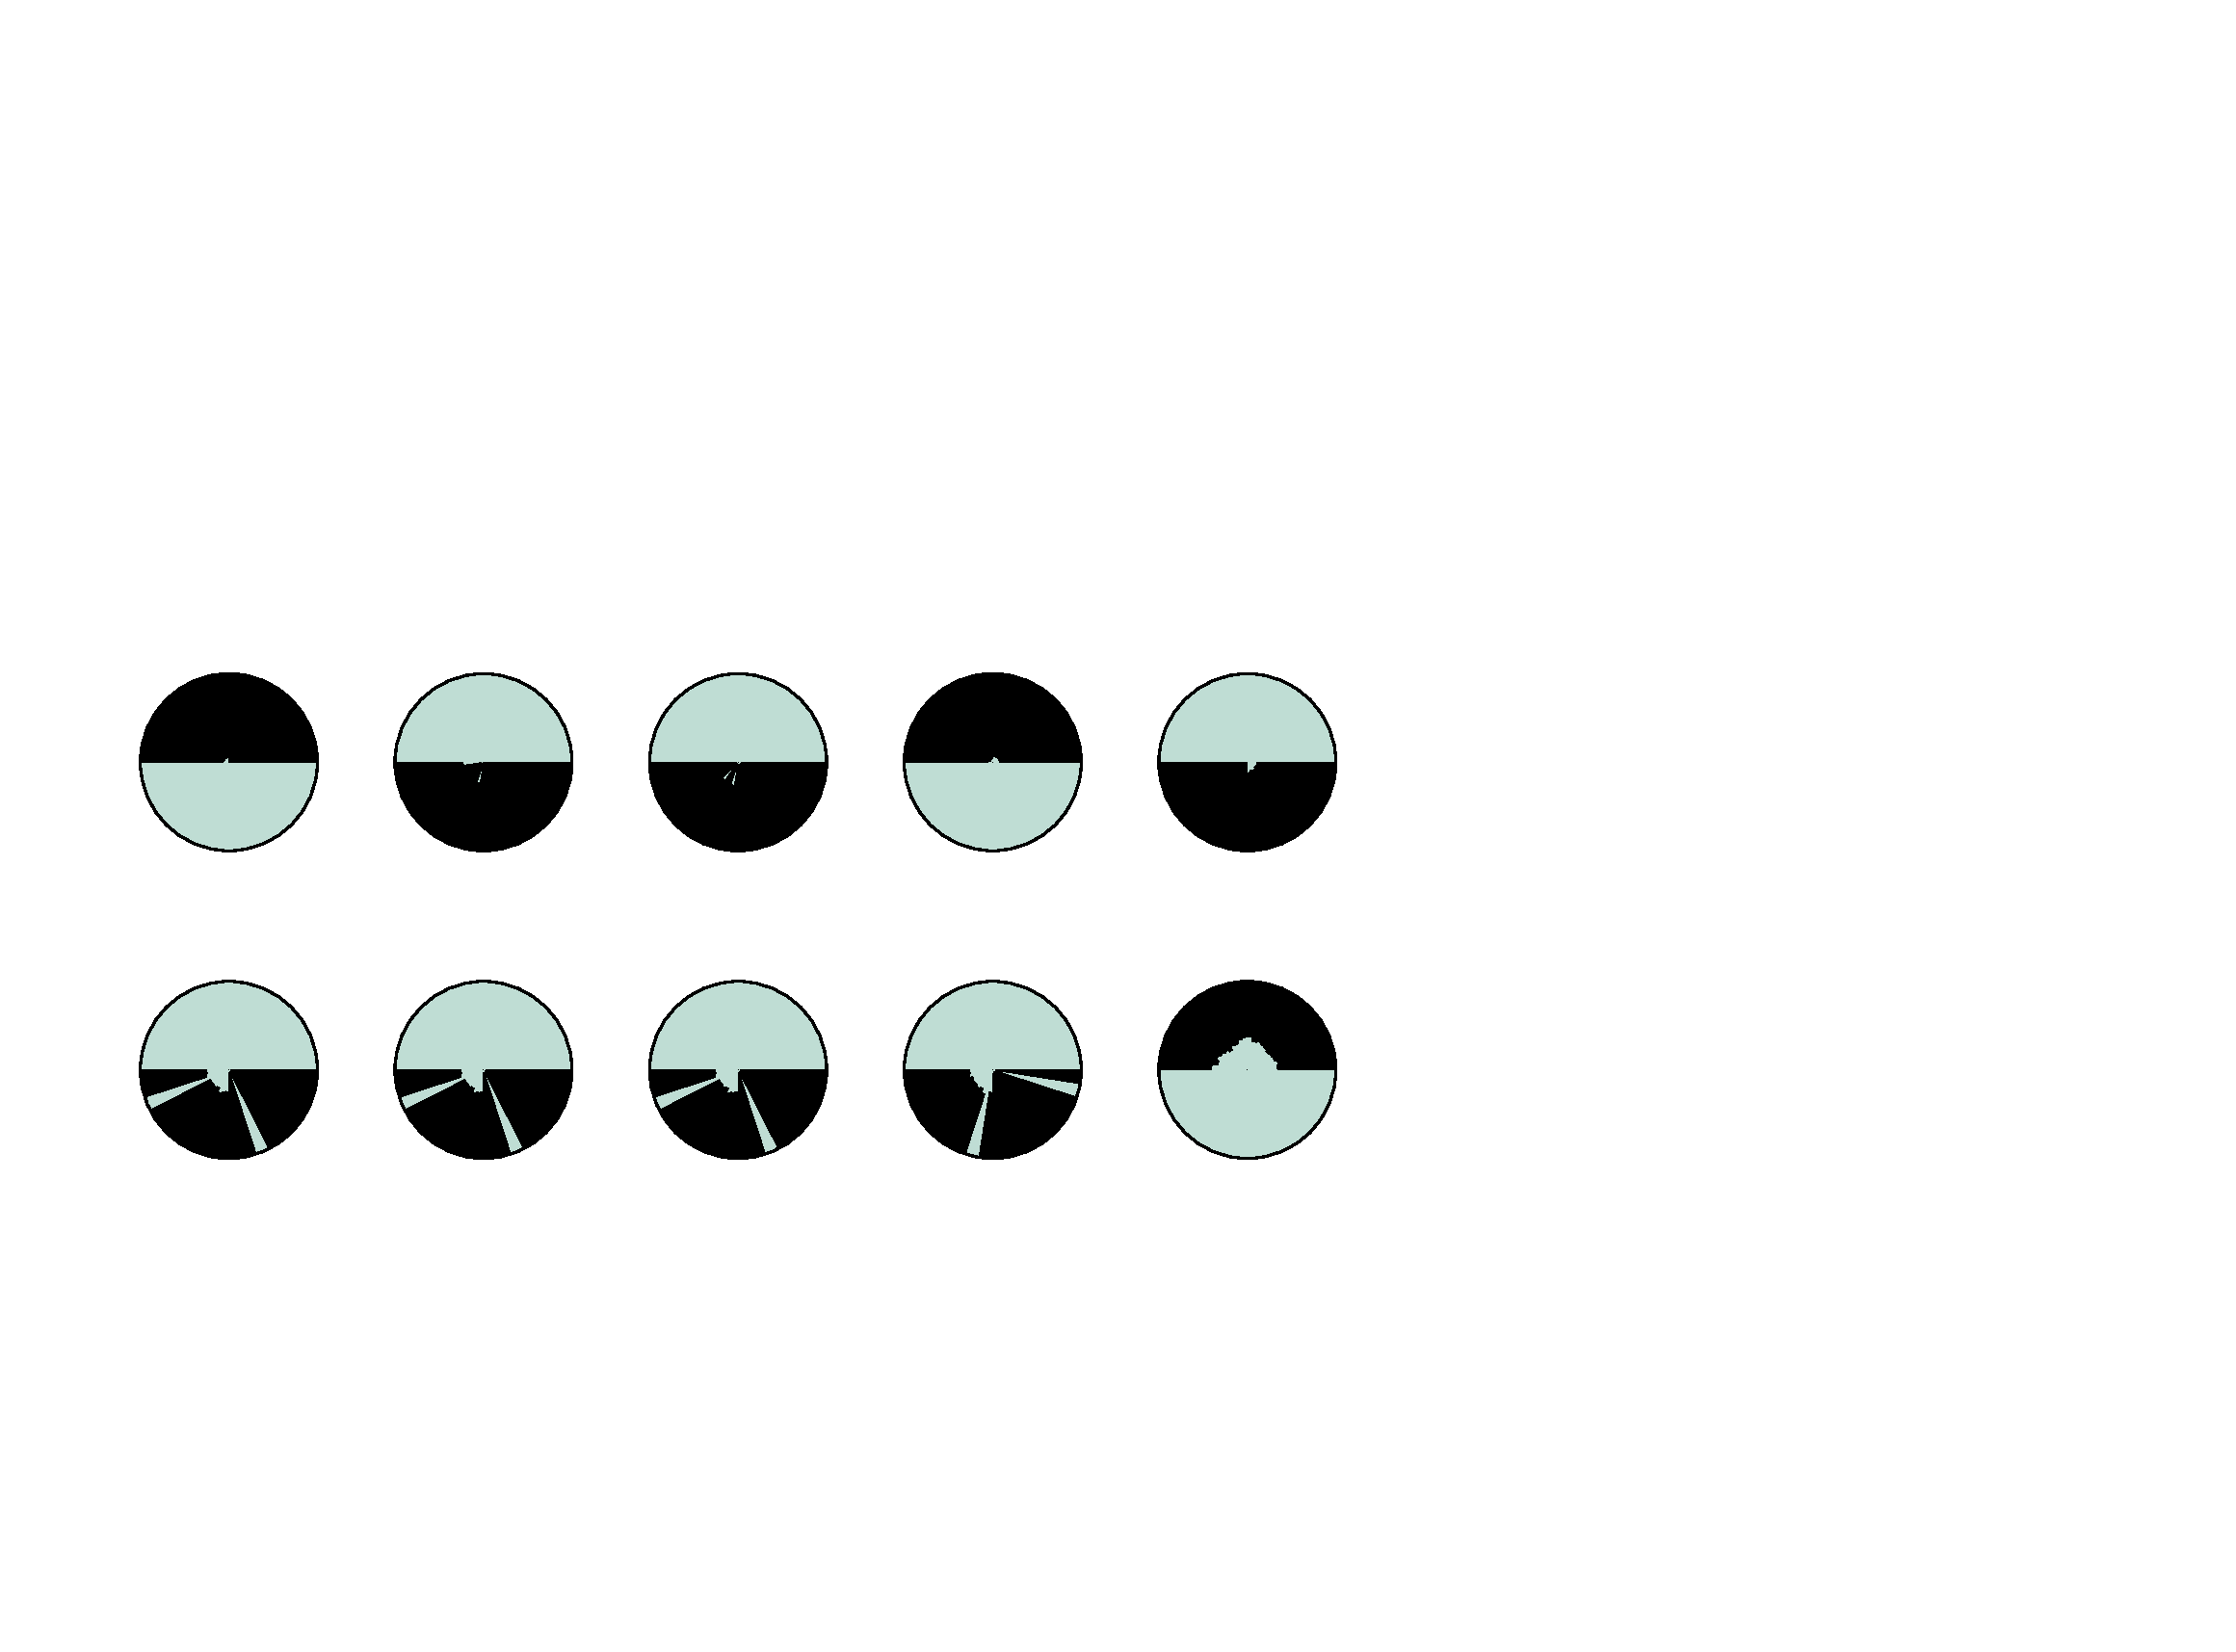
\includegraphics[width=\linewidth]{infuse/usecase1b}
\caption[The clinical researchers found an interesting pattern among
the glyphs.]{
The clinical researchers found an interesting pattern among
the glyphs indicating non-overlap of feature selection algorithm results.
These features were highly ranked by 2 of the 4 feature algorithms,
and unranked by the other 2, resulting in glyphs that resemble half-circles.
}
\label{fig:usecase1}
\end{figure}

% !TEX root = ../featureselection.tex

\section{Future Work and Conclusion}
There remains a great deal of research to further improve the analytical process of predictive modelers. \infuse only focuses on the feature selection step of predictive modeling. Each of the other steps would benefit from a visual interface to explore and parameterize the pipeline as well.

The search capabilities also have room for improvement by allowing more complex queries like features with a given range of ranks or features picked by a given algorithm, which would ease the task of finding relevant features for a user.
Also, expanding the range of the search box to filter also in the Feature View may reduce the number of overlapping glyphs in the scatterplot view.
Other clutter reduction techniques could also be available to users, such as a semantic zooming overlap resolution strategy that can jitter glyphs that overlap when the view is zoomed in.

Finally, to date, this tool has been used extensively for predictive modeling on clinical data.
However, \infuse was designed to be domain-independent and can easily be used for other domains in need of high-dimensional predictive modeling.  Our future work includes additional case studies in other domains to ensure the robustness of our tools.  This would also give the opportunity to explore the scalability of the design.  Typically, the number of cross-validation folds is not more than ten.  However, certain analysts may wish to compare a larger number of feature selection algorithms which would decrease the amount of space available per algorithm in the glyph.  While similarly-ranked features would still appear visually alike, it may become difficult to identify certain algorithms or folds without the help of interaction.  The overall number of features also plays a role in scalability concerns.

In conclusion, predictive modeling techniques are increasingly being used by data scientists to understand the probability of predicted outcomes.  We present \infuse, a tool that
lets users interactively create predictive models.  Typically, the predictive modeling pipeline leaves users out of the loop, and the algorithms operate as a black box.  By giving users the power to interact with the results of feature selection, cross validation folds, and classifiers, \infuse has shown promise to improve the predictive models of analysts.  We further demonstrated how our system can lead to important insights in a case study involving clinical researchers predicting patient outcomes from electronic medical records.


%% if specified like this the section will be ommitted in review mode
% \acknowledgments{
The authors thank Kenney Ng for providing
his expertise in predictive modeling.
The authors also thank the anonymous healthcare institution
who provided the data for the clinical researchers experiments.
% }


% \bibliographystyle{abbrvnat}
% \bibliography{progressive_vis}
% \end{document}
